% vim:spell:spl=en_gb:fenc=utf-8:et:sw=4:ts=4:sts=4
%
% This document has been prepared for use with pdfLaTeX 

% The margins produced by standard classes (ar ticle.cls, report.cls, book.cls) 
% are often deemed too wide by Europeans using A4 paper. The classes in the 
% Koma-Script bundle (scrartcl.cls, scrrepr t.cls, scrbook.cls) are specially
% designed for European and German typography (komascript.de):
\documentclass[11pt,bibliography=totoc,index=totoc]{scrbook}   % paper=a4 is default, 11pt is actually also default

% dmthesis.sty : LaTeX style for my Master's Theses
% created by :
%    Dan Michael Olsen Heggø
%    (danmichaelo@gmail.com)

%\typeout{Hello world}

\KOMAoptions{parskip=half, BCOR=7.5mm, DIV=11, mpinclude=false}  % skip margin notes
% DIV=11 gir oss i utg. pkt. 152.73 mm tekstbredde og 216 mm teksthøyde.
% men vi trekker fra 7.5 mm som forsvinner i innbindingen (BCOR)
% og står igjen med 147.26 mm tekstbredde.

\usepackage[greek,british]{babel}		% Localization
\usepackage[utf8]{inputenc}				% For typing accentuated characters directly

%\usepackage{kpfonts}                   % kp is nice for text, but the math isn't acceptable 
\usepackage{lmodern}                    % Use fully scalable fonts
\usepackage[T1]{fontenc}            	% T1 contains the french guillements.. 
\usepackage{lettrine}

%%%%%%%%%%%%%%%%%%%%%%%%%%%%%%%%%%%
% MATH:

\usepackage{amsmath,amsthm,amssymb}		% AMS Math support
\usepackage{empheq,mathtools}
\usepackage{siunitx} 					% For consistent units. Includes upright mu.
										% Must be loaded after amssymb

\renewcommand{\vec}[1]{\boldsymbol{\mathrm{#1}}} 	% Use bold vectors
\newcommand{\nvec}[1]{\mathrm{#1}} 	                % matrices, etc.. 


%%%%%%%%%%%%%%%%%%%%%%%%%%%%%%%%%%%
% FONT:

%\usepackage{kmath,kerkis}          	% The order of the packages matters; 
                                    	% kmath changes the default text font
                                    	% Must be loaded after amsmath

%%%%%%%%%%%%%%%%%%%%%%%%%%%%%%%%%%%
% Figures and tables:

\usepackage[usenames,dvipsnames]{color}	% usenames + dvipsnames gives us 66 predefined colors. 
\usepackage{graphicx}					% Graphicx is the extended graphics package.
%\graphicspath{{imgs/}{moreimgs/}}
\DeclareGraphicsExtensions{.pdf,.png,.jpg} 	% specifies the behaviour of the system when no 
											% file extension is specified in the argument
\usepackage{subfigure} 					% for subfigures

%\usepackage{wrapfig} 					% for \begin{wrapfigure}

% Print figure and table labels in a smaller font, and print `Figure:' and `Table:' in boldface:
\usepackage[margin=10pt,font=small,labelfont=bf,labelsep=colon,format=plain,indention=.5cm]{caption}


\usepackage{booktabs}					% production quality tables
\usepackage{threeparttable}				% for placing footnotes under tables
%\usepackage{multirow} 					% for multi-row table cells

\usepackage{framed} % for drafting only

%%%%%%%%%%%%%%%%%%%%%%%%%%%%%%%%%%%
% CHEMISTRY :

%\usepackage[version=3]{mhchem}			% Latest version: 3.07


%%%%%%%%%%%%%%%%%%%%%%%%%%%%%%%%%%%
% MISC :

\usepackage{fancybox}					% For boxed environments
\usepackage{layout}						% For page layout debug (\layout)
\usepackage{soul}                       % For highlighting (in the draft phase)


% Note that LaTeX can only draw lines with slope = x/y, where x and y have integer values from −6 through 6.
\newcommand{\crossbox}[1]{ %
    \setlength{\unitlength}{#1}
    \begin{picture}(1,1)(0,0)
       \put(0,0){\framebox(1,1){ }}
       \put(0,0){\line(1,1){1}}         % (slope x, slope y){length}
       \put(1,0){\line(-1,1){1}}        % (slope x, slope y){length}
    \end{picture} %
    }



%%%%%%%%%%%%%%%%%%%%%%%%%%%%%%%%%%%
% BIBLIOGRAPHY :
\usepackage[safeinputenc,backend=biber,hyperref=true,sorting=none,style=numeric]{biblatex}


%%%%%%%%%%%%%%%%%%%%%%%%%%%%%%%%%%%
% HYPERREF :
\usepackage{hyperref} 	% Make sure it comes last of your loaded packages, 
						% to give it a fighting chance of not being over-written, 
						% since its job is to redefine many LATEX commands.
						% It is preferable to load it after biblatex.
\hypersetup{pdftex,unicode, 
    colorlinks=true,linkcolor=blue,citecolor=blue,urlcolor=blue,    
    pdfdisplaydoctitle=true, 
    bookmarksopen=true,bookmarksopenlevel=2,        
    pdfauthor   = {Dan Michael Olsen Heggø},            
    pdftitle    = {Not Set Yet},                         
    pdfkeywords = {phosphorus, diffusion, silicon, solar cells, master thesis}
}




\usepackage{makeidx}
\makeindex

% Macros
\newcommand{\ksorb}{\ensuremath{\psi^{\mathrm{KS}}}}

% Temporary premable-stuff:
\usepackage[marginpar]{todo}
\newcommand{\comment}[1]{\hl{#1}}
%\usepackage{layouts}

% Bibliography:
\bibliography{bibliography/master}

% Title page (koma-script options):
%\titlehead{Titlehead}
%\subject{Subject}
%\usepackage{titling}
%\subtitle{Subtitle}
%\publishers{Pub}

\newcommand{\vasp}{{\texttt{VASP}}} % eller \sc?
\newcommand{\vesta}{{\texttt{VESTA}}} % eller \sc?
\newcommand{\vmd}{{\texttt{VMD}}} % eller \sc?

\begin{document}
\frontmatter
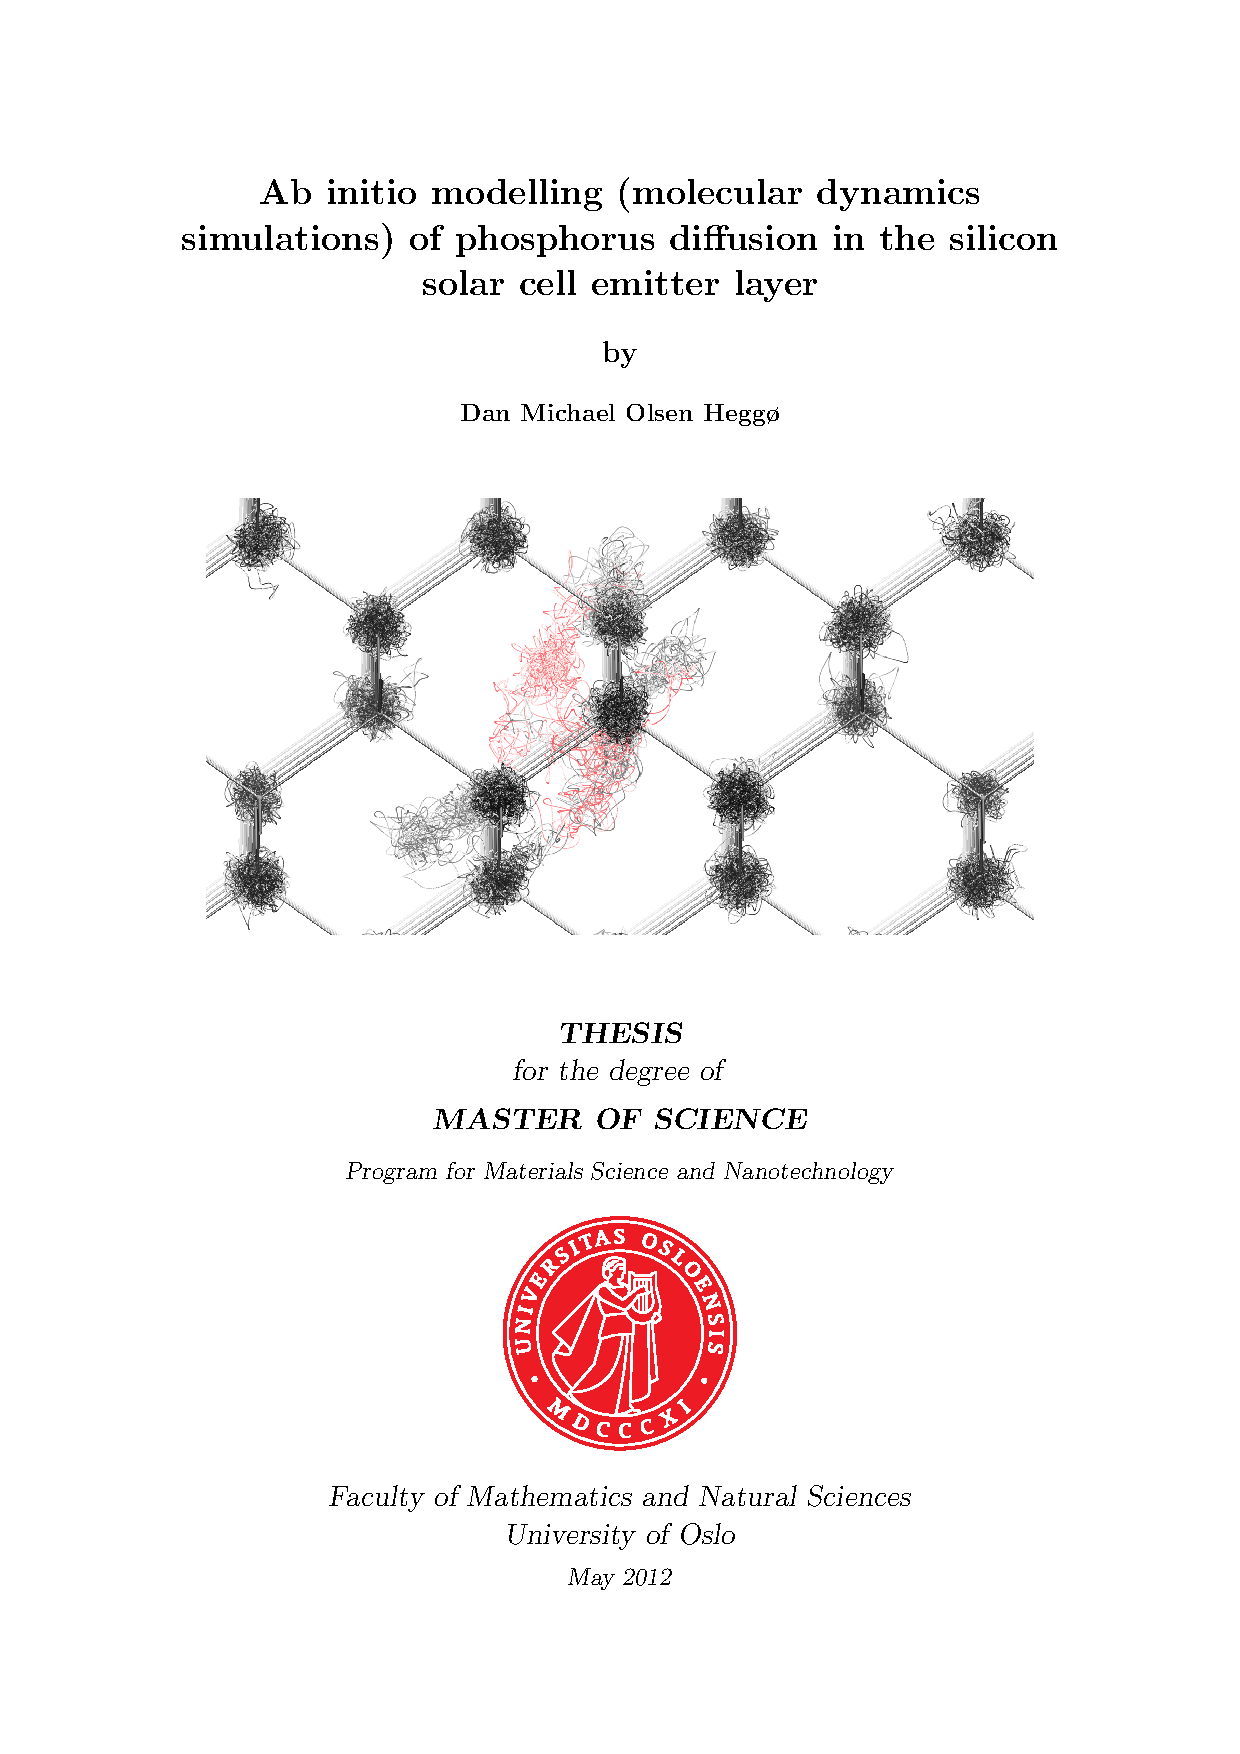
\includepdf{frontpage/frontpage.pdf}

Acknowledgement

Abstract

Sammendrag på norsk

% pdflatex -v | head -n1
Set with the help of {\LaTeXe} and {\KOMAScript}.

%Grasping the amount of work behind this possibility is hard,
%generations before you have laid out the theories of quantum mechanics and of
%solid state physics, prepared a huge library of crystallographic data, 
%developed computing power at a remarkable pace, and written millions of lines
%of computer code. Sometimes you feel very tiny.

\tableofcontents

\mainmatter
\pagestyle{scrheadings}

\part{Background, theory and preparations}

\chapter{Background} % Prolegomena

\section{Introduction}

%\lettrine[lines=3, findent=.2em, slope=-0.5em, nindent=0pt]{W}{hile}
%I personally have no preference for materials over any other matter,
%it happened that I ended up in materials science, the study of 


%I was driven into this discipline by my interest in materials for 

utilisation of some of the \SI{120000}{\tera\watt}
of net power we receive from the Sun -- most of which is `spilled' today. 

Molecular dynamics with an \textit{ab initio} potential, such as one obtained from DFT calculations, is very tempting from a theoretical point of view (finne kilder), but has generally been considered unfeasable from a practical point of view due to the great computational cost involved.
Modeling at the \textit{ab initio}, while 


I'm grateful to the developers of the VASP software, who provided me with new potentials that decreased the computing time considerably. These are described further in section \ref{sec:pseudopot}

This work was started without knowing \textit{a priori} if simulations at the \textit{ab initio} level could be carried out with simulation times long enough to obtain useful statistics, but with new potentials and \ldots we found it worthwhile to test.

A privilege with studying phosphorus in silicon is that there exists a wealth of experimental and theoretical results from more 
than 60 years\footnote{
  Silicon semiconductor technology took it first infant steps right before world war II, with for instance
  the discovery of the p-n junction (then called `PN barrier') often attribtued to R.S Ohl (U.S. patent 2402662, 1939),
  and the understanding and development gained speed in the early 50s. In a 1953 patent by P. Robsin, the process of 
  diffusion to form a junction is described (U.S. patent 2823149, 1953), and in a 1955 patent by Ross (2862160), 
  phosphorus is mentioned as a donor. But I'm not sure just when phosphorus was first introduced.
} of studies on this system. 
, data that can be used to test our models. 
For example, there are the classic, often-cited reviews on diffusion of dopants in silicon by (Fahey:198) and (Hu:1994). And the PhD thesis of (Bentzen:2006) provides an up-to-date account of the diffusion behaviour of phosphorus in the specific case of the very highly doped emitter layer.

As an introduction, table \ref{tb:si} presents some key properties of silicon,

\begin{table}[htb]
  \centering
  \begin{tabular}{lll}\toprule
     & 300~K & 1100~K\\
     Crystal structure & Diamond  \\ 
     Lattice constant / Å  & 5.43086 \cite{Ghandhi:1994}, 5.43072 $\pm$ 0.00004 Å at \SI{25}{\celsius} \cite{Smakula:1955} \\
     Distance between neighboring atoms / Å & 2.35163 \\
     Atomic density & \SI{4.99441e22}{\per\centi\metre\cubed} \\
     Melting point & \SI{1685}{\kelvin} / \SI{1412}{\kelvin} \\
     Thermal coefficient of expansion & \SI{2.33e-6}{\per\kelvin} & \SI{4.5e-6}{\per\kelvin} \\\bottomrule
  \end{tabular}
  \caption{Some key properties of silicon (Har ikke helt bestemt hvilke som bør være med her)}
  \label{tb:si}
\end{table} 


\section{The power of the sun}
\lettrine[lines=3,slope=0pt,nindent=0pt,lraise=0.12]{Q}uite
stabily, our Sun emits about 383 yottawatts of radiative power [SOURCE]. 
8 light minutes away, our small, blue planet receives about 100 petawatts ($10^{17}$
) of radiative power [CHECK].
In thermodynamic terms, the radiation is an
energy flux of relatively low entropy, meaning that it's easier to utilize
than lower-entropy energy fluxes such as heat. It is a `high-quality' energy
flux, an energy flux that is the starting point for all processes on earth
but those utilising geothermal energy. From a logical point of view, it makes
perfect sense to utilise solar energy directly instead of one of its
`derivates', like wind, hydro, etc. Yet, there is one issue with solar
energy: it's diluted, at least compared with the energy content of fossil
fuels that we are so spoiled with. One litre of gasoline contains about 9.5 kWh of
energy\footnote{\url{http://www.ocean.washington.edu/courses/envir215/energynumbers.pdf}}.

To get a feeling for this number, remember that one kilowatt-hour of electric power 
is roughly one and a half hour of horse-power. Man, not being as strong as a
horse, can only sustain about one tenth of a horsepower over time, meaning that a 
full working day amounts to less than one kilowatt-hour, further meaning that 
roughly 10 hard working days can be replaced by a single litre of gasoline in terms
of energy content. 

How about solar power? In a solar-rich area, we receive the same amount of energy 
over 9.5 square metres in one hour. That's why we say that solar power is rather
\emph{area-intensive}.

Blabla. solceller må derfor være tynnest mulig og mest mulig effektiv.

solar constant: 

$1366\pm 40$ W/m$^2$. The yearly variation of about $\pm 3\%$ 
due to the variation of Earth's distance to the Sun during the year, is much
larger than the known variations in the radiation itself.\footnote{
Phillips, Kenneth J. H. (1995). Guide to the Sun. Cambridge University Press. 
pp. 14–15, 34–38. ISBN 9780521397889.
\url{http://www.pmodwrc.ch/pmod.php?topic=tsi/composite/SolarConstant}
\url{http://books.google.com/books?id=YEN9fC9tbEgC}
}

solar constant $1353\pm 45$ W/m$^2$ (Marstein forelesningsnotater)
. de Vos, s. 19: 1353, pm 3.5\%.

About $5.8\times 10^{17}$ photons/sec/cm$^2$ reach the outer atmosphere, while
some $10^{17}$ survive through the atmosphere.\footnote{Solar Cells (Backus)}

\section{The silicon solar cell}

Silicon doped with a donor, like phosphorus, is called n-Si. Highly-doped areas in the proximity of the metal contacts are often referred to as n+ or n++.

The contact resistivity $\rho_c$ depends strongly on the doping concentration $N_D$, as reviewed by Schröder\cite{Schroder:1984}. 
If the metal contacts take up 5\% of the cell surface, a contact resistance $\rho_c < \SI{2e-3}{\ohm\centi\metre\squared}$ is required to not degrade the output power by more than 0.5\%. This in turn requires a doping concentration $N_D > \SI{1e19}{\per\centi\metre\cubed}$,but even higher doping concentrations is required if the area occupied by metal contacts is reduced, or if used in concentrator cells with higher power.

\subsection{Short solar cell history (kan kanskje sløyfes)}

The ``Effect of Light on Selenium during the passage of an Electric Current''
was described by W. Smith in 1873\cite{Smith:1873}.

1876 eller 1877 (?) - W.G. Adams and R.E. Day observed the photovoltaic effect in solidified 
selenium, and published a paper on the selenium cell. 'The action of light 
on selenium,'\cite{Adams:1876}

The first known solar cell was built in 1883 by Charles Fritts who coated the
semiconductor selenium with a thin layer of gold to form a junction.

Russell Ohl, in 1939, discovered the PN barrier (or as it became known, 
the “P–N junction”). He is generally recognized for patenting the modern solar 
cell (US Patent 2402662, "Light sensitive device"). Ohl was a notable 
semiconductor researcher prior to the invention of the transistor. 

Solar cells later became practical for power uses after Russell Ohl's 1941 
development of silicon p/n junction cells that reached efficiencies above 
5\% by the 1950s/1960s.

%Multicrystalline silicon (mc-Si) wafers are widely used for man- 
%ufacturing of solar cells due to their relatively low price and high 
%performance. is responsible for the kink-and-tail profile [11–13]. The effective 
%diffusivities describing the high and low concentration regions of 


%Today, silicon-based solar cells are most widely used because of their
%relatively low price and high performance. Even cheaper are many of the thin
%film approaches, but at the cost of lower performance, meaning larger areal
%cost. The most popular also make use of scarce elements, which mean that such
%solar cells cannot play a major part of a renewable energy scenario.

%While solar cells today are commonly quoted as being to expensive, a remarkable
%project initiated by the Barefoot College in India have shown that even the
%poorest of the poor can often reduce their expenses by replacing kerosene with
%silicon solar cell based lightning.

%The main problem is of course that fossil fuel is underpriced.

%Even so, there is a broad hope for a great increase in solar cell performance in
%the coming years. How is it to be achieved? From a modelling point of view we
%can study both materials that have never been tested in the real world. Can
%computer modelling give us insight into what the ideal solar cell material would
%be?


\section{Diffusion and diffusivity}\label{sec:Diffusion}

Diffusion\index{diffusion} is the redistribution of atoms\footnote{I will only be concerned with atoms here, but the concept of diffusion also applies to other small particles such as molecules, viruses and bacteria} due to their thermal motion. 
Such redistribution occurs in all materials, but at a negligible rate at temperatures considerably below the melting point of the material.
For silicon, with a melting point of \SI{1414}{\celsius}, diffusion is negligible at room temperature, 
but significant at elevated temperatures, and controlled diffusion is commonly carried out at temperatures 
of about 800-\SI{1000}{\celsius}. 

How do we describe and model diffusion?
As is not uncommon in physics, different pictures exist for different scales of interest. 
When it comes to describing diffusion, two main pictures exists: the continuum picture and the atomistic picture. 
Since materials consists of atoms, it is clear that the most fundamental picture of diffusion should be an atomistic one.
But a description involving every single atom becomes highly impractical on a macroscopic scale\footnote{\comment{Clarify macroscopic / microscopic?}
}, in which it becomes more practical to invoke a viscous fluid model in which the atoms are smoothed out into a continuum.
The two pictures can be connected through parameters known as diffusion coefficients in order to produce integral diffusion models,
but the diffusion coefficients are also commonly obtained empirically.

\subsection{The continuum picture}

Following Joseph Fourier's 1822 treatise on heat diffusion\cite{Fourier:1822} and Georg Ohm's 1827 work on `electricity diffusion' (Ohm's law),\cite{Ohm:1827} Adolf Fick presented his phenomenological description of `mass diffusion' in 
1855.\cite{Fick:1855}
In this picture, a species with concentration $c(\vec{r})$ will flow in the opposite direction of the concentration gradient of that species, $\nabla c(\vec{r})$. That is, it will show a flux,
\begin{equation}
  \vec{J}(\vec{r},t) = - D \nabla c(\vec{r},t).
  \label{eq:ficks1st}
\end{equation}
This relationship between the concentration gradient and the flux is known as Fick's first law, and the constant of proportionality $D$ is known as the coefficient of diffusion or \emph{diffusivity}\index{diffusivity} for the species in question. 
Often reported in units of \si{\metre\squared\per\second} or \si{\centi\metre\squared\per\second}, the diffusivity is in general a tensor, but it reduces to a scalar in cubic crystals. 
In general the diffusivity of species $i$ will depend on both the concentration of the same species $c_i$ and of other species $c_j$, on temperature, pressure, crystal defects and other factors that will be quickly discussed below.

If $G$ and $R$ are the generation and recombination rates for the species in question, a continuity equation could be set up as
\begin{equation}
    \frac{\partial c}{\partial t} = -\nabla \vec{J} + G - R
  \label{eq:continuity}
\end{equation}
In the absences of sinks and sources ($G=R=0$), the continuity equation combined with Fick's first law forms what is known as Fick's second law,
\begin{equation}
    \frac{\partial c}{\partial t} = \nabla (D \nabla c) = D \nabla^2 c
  \label{eq:ficks2nd}
\end{equation}
where the last equality is true only when $D$ is independent of position (via the concentration).

The picture is slightly complicated by the fact that the diffusivity $D$ itself may vary with the concentration $c$.
\index{diffusivity!dependence on concentration}
For the diffusivity of species at very low concentrations, such as dopants, this concentration dependence is generally negligible, but at high concentrations, such as the typical phosphorus concentrations in the solar cell emitter layer, the effect may be quite significant.
As an example, A. Bentzen has obtained the concentration dependence of the phosphorus diffusion coefficient over a large range of concentrations using Boltzmann-Matano analysis of experimental data at \SI{890}{\celsius}. 
From the intrinsic value of about \SI{4e-14}{\centi\metre\squared\per\second}, his diffusivity increases slowly up to a maximum of \SI{1e-13}{\centi\metre\squared\per\second} at a phosphorus concentration of \SI{e19}{\per\centi\metre\cubed}, before it dips down to \SI{1e-14}{\centi\metre\squared\per\second} at \SI{e20}{\per\centi\metre\cubed}, before it increases again.\cite{Bentzen:2006} Concentration gradients will nevertheless not be considered in this work.\comment{upresist?}

\index{diffusivity!dependence on temperature}
The diffusivity depends strongly on the temperature, and the temperature dependence found from experiments often takes the simple Arrhenius form,
\begin{equation}
  D(T) = D_0 \e^{-E_a/kT}
\end{equation}
defined by a prefactor $D_0$ and an activation energy $E_a$. 
Taking the logarithm on both sides, we see that $\ln D$ as a function of $1/kT$ forms a straight line with slope $-E_a$ and interceipt $\ln D_0$. 
\begin{equation}
  \ln D = \ln D_0 - E_a (kT)^{-1}
\end{equation}
The parameters $D_0$ and $E_a$ can thus easily be extracted if a good fit can be made to a straight line.

%While diffusion is an activated process, the activation energy obtained from experiments will in general not result from a single activated process, but rather a mix of different processes, and this necessarily complicates the determination of the processes involved.
%In fortunate cases, a single process may be dominating.

%Since the diffusion of atoms in an crystal is though of as an activated process with an activation energy $E_a$, the temperature dependence will often take the simple Arrhenius-form,

As mentioned, the diffusivity may also depend on other factors, such as crystal defects, pressure, et cetera, that will not be touched upon in this work, but these are discussed by e.g. Pichler.\cite{Pichler:2004}

\subsection{The atomistic picture}

In the continuum picture, the diffusion coefficients are just empirical parameters, and we have to invoke a model involving atoms to explain them.

From the Gaussian diffusion outwards from a point,
\begin{equation}
    c(x,t) = \frac{n}{\sqrt{4\pi D}} \e^{-x^2/4Dt} / \sqrt{t},
\end{equation}
\comment{SJEKK OPP}
Einstein related the displacement along the $x$ axis, $\lambda_x$, to the diffusivity\cite{Einstein:1905},
\begin{equation}
    \lambda_x = \sqrt{x^2} = \sqrt{2Dt}
  \label{eq:einsteinRelationSimple}
\end{equation}
Na\"{\i}vely, the diffusion coefficient of a species can thus be found from a knowledge of the displacement of all atoms of that species,
and this is actually the approach followed in molecular dynamics simulations.
While it's a tempting approach, and also the one followed in this work, it should not come to a surprise that simulating a large number of atoms over a sufficient amount of time is a computationally demanding task, and for many systems it's just not feasible. 
A short discussion of other approaches is therefore in place, especially since these to a large degree have formed the way we understand and describe diffusion.

In the solid phase, very little diffusion occurs compared to the liquid or gas phase. 
In a crystal, the atoms remain at given lattice sites most of the time.
At a finite temperature $T$, the atoms will have kinetic energies according to a Boltzmann distribution for that temperature,
and since the atoms are `trapped' by the neighbouring atoms this energy goes into vibrations. 
If, however, an atom obtain a kinetic energy larger than a given treshold energy, it can migrate (`jump') into another site.
This is an example of what is called an \emph{activated process}, and the treshold energy is called an activation energy, $E_a$.
In general there is not just one diffusion mechanism involved, and the value for the activation energy obtained by experiment or simulation is a weighted average over all possible mechanisms.
One mechanism may, however, be the dominating one. In the case of phosphorus in silicon, there is a general consensus that interstial-mediated diffusion is the dominating mechanism. \comment{KILDER!}

Now, from the Boltzmann distribution (see \ldots), the fraction of atoms having a kinetic energy greater than a given energy $E_a$ is $\e^{-E_a/KT}$, and so the probability for a jump to happen is just $\e^{-E_a/kT}$. 

In a simple model, we can estimate the number of jumps per second \comment{PER ATOM?} by multiplying this probability by the attempt frequency $\nu$,
\begin{equation}
  \Gamma = \nu \e^{-E_a/kT}
  \label{eq:jumpfreq-est}
\end{equation}
For a rough estimate, we may take the frequency to be \SI{e13}{\hertz}, a typical textbook value for the vibration of atoms in a crystal at room temperature.
As seen in fig. \ref{fig:simple-vibration}, the atoms may be described roughly as vibrating at frequencies of this order of magnitude, although the motion is of course much more complicated than a simple harmonic motion. Otherwise we would not need \emph{simulation}.

\begin{figure}[htbp]
  \begin{center}
    \includegraphics{../figures/md_test_fft}
  \end{center}
  \caption{
    Simulated motion of a silicon atom in a 64-atom supercell at 1400 K (solid line), 
    with a least square fit to a function $f(t) = a \cos[(2\pi f)t + c] + d$ (dashed line). 
    The fitted frequency is $f=\SI{3e12}{\hertz}$, corresponding to a period of 0.3~ps.
  }
  \label{fig:simple-vibration}
\end{figure}

\begin{figure}[htbp]
  \begin{center}
    \includegraphics{../figures/jump_frequency}
  \end{center}
  \caption{Estimated jump frequency from \eqref{eq:jumpfreq-est} with $\nu=\SI{e13}{\hertz}$.}
  \label{fig:jumpfreq-est}
\end{figure}




At the microscopic scale, an atom in a crystal will not move freely, but vibrate in a unharmonic and complicated way in the potential well of the other atoms. 
If its motion is averaged over the timescale of the vibrations, which are in the order of pico-seconds, it will appear more or less fixed in space. 
Every now or then, it will, however, obtain enough energy to `jump' to a different position.

\begin{figure}[htbp]
  \begin{center}
    \includegraphics{../figures/md_test_diffusion_jump}
  \end{center}
  \caption{A `jump' from one lattice site to another. The red line is a symmetric running mean over 0.5 ps followed by a symmetric running median over 2.0 ps.}
  \label{fig:../figures/md_test_diffusion_jump}
\end{figure}

The diffusion coefficient in liquids is typically of the order of $10^{-7}$ cm2/s,
while in solids its magnitudes smaller, typically of the order of $10^{-11}$ cm2/s. \comment{[kilder!]}


The diffusion coefficient in crystals with a cubic lattice should be isotropic.

\section{The case of phosphorus diffusion in silicon}\label{sec:PinSi}

\subsection{How much phosphorus go into silicon and where does it go?}

According to the standard phosphorus-silicon binary phase diagram, more than 2\% P can be solved in silicon at temperatures between \SI{1350}{\kelvin} and \SI{1500}{\kelvin} without the formation of new phases, and even at 1000 K about half a percent can be solved.\cite{PSiPhaseDiagram} 

Sheet resistivity and Hall effect measurements have shown that below about 2–\SI{3e20}{\per\centi\metre\cubed} (or 0.4-0.6\%), the density of electrically active dopants in properly annealed samples follow the chemical concentration of phosphorus closely, but above such a concentration, the density of electrically active dopants $n_e$ plateau.\cite{Tannenbaum:1961}
A concentration of about half a percent therefore seems to be the maximum solubility of unclustered P,\cite{Solmi:1998} but higher concentrations
%(reached above about \SI{750}{\celsius},\cite{Solmi:1996} and)
are common in the heavily doped emitter layer in solar cells.\cite{Bentzen:2006b}
The exact nature of the ``extra'', inactive phosphorus is not known, but a mix of SiP precipitates and mobile P defects have been suggested.\cite{Armigliato:1976}\cite{Solmi:1996} 
%When the concentration of phosphorus exceeds the solid solubility,  orthorhombic crystallites of silicon monophosphide (SiP) will start to precipitate within the silicon matrix,\cite{Arimgliato:1976} 

The atomic radii of silicon and phosphorus are 1.17 and 1.10~Å, respectively.
Due to the similar size, it was early assumed that phosphorus occupy mainly substitutional lattice sites, and this was confirmed by some of the first 

A solid solution of phosphorus in silicon is therefore expected to have a slightly smaller lattice parameter than pure silicon.
That a small shrinkage takes place on in-diffusion of phosphorus into silicon was first described by Pearson and Bardeen in 1948, who reported a slight lattice constant shrinkage of some 0.02 \% when adding some 0.5 at\% phosphorus,\cite{Pearson:1949} 

Comparing Pauling's tetrahedral covalent atomic radii (Kittel, p. 105), $(V_{\text{Si}}-V_{\text{P}})/V_{\text{Si}} = -0.17$.
Using effective-mass theory, Pajot and Stoneham found a volume contraction, $\Delta V/V_{\text{Si}} = -0.08$.

The solid solubility of phosphorus is in the order of 1\%. After in-diffusion of phosphorus into silicon , an annealing step 
After proper annealing, the density of electrically active dopants can reach about 2–\SI{3e20}{\per\centi\metre\cubed}, or 0.4--0.6\%,
or even \SI{4e20}{\per\centi\metre\cubed} for annealing temperatures higher than those used in normal solar cell processing.

but at temperatures above \SI{750}{\celsius}, 
however, the limit of solunlieven more phosphorus appears to be solv

Newero\cite{Borisenko:1987} and \cite{Safarian:2011} 

The tetrahedral structure of the silicon atoms is a relatively open one, with a spherical packing density of only $\pi\sqrt{3}/16\approx 0.34$.\footnote{Close-packed spheres have a spherical packing density of $\pi/3\sqrt{2} \approx 0.74$.}
This makes possible many different interstitial configurations, and also interstitial diffusion

In a 2003 nudged elastic band study, Liu et al identified several insterstitial configurations for phosphorus in silicon.
They found the most stable one to be a [110] dumbbell configuration, $P_i^X$, in which a Si-P pair shares a single lattice site, oriented in the [110] direction. The centre of the pair is not located directly on the lattice site, but is translated a short distance in the [001] direction. This gives rise to the `dumbbell' name and the low $C_1$ symmetry.
Further they identified a hexagonal configuration, $P_i^H$, and a [100] dumbell-like configuration, $P_i^s$.

%%%%%%%%%%%%%%%%%%%%%%%%%%%%%%%%%%%%%%%%%%%%%%%%%%%%%%%%%%%%%%%%%%%%%%%%%%%%%%
%%%%%%%%%%%%%%%%%%%%%%%%%%%%%%%%%%%%%%%%%%%%%%%%%%%%%%%%%%%%%%%%%%%%%%%%%%%%%%
%
\chapter{Density Functional Theory}\label{cha:dft}
%
%%%%%%%%%%%%%%%%%%%%%%%%%%%%%%%%%%%%%%%%%%%%%%%%%%%%%%%%%%%%%%%%%%%%%%%%%%%%%%
%%%%%%%%%%%%%%%%%%%%%%%%%%%%%%%%%%%%%%%%%%%%%%%%%%%%%%%%%%%%%%%%%%%%%%%%%%%%%%

This chapter consists of two parts. The short sections \ref{sec:materials}--\ref{sec:forcetheorem} give a general presentation of density functional theory (DFT), 
while the lengthy section \ref{sec:parameters} is concerned with the practical choices made in the application of the theory in this specific work.

The aim of the first part has not been to \emph{introduce} DFT,\footnote{
A good practical introduction is given by Scholl(2009)\cite{Scholl:2009}, while a more theoretical and authoritative introduction is given by Parr(1994)\cite{Parr:1994}.
Chapter 12 in Kantorovich(2004)\cite{Kantorovich:2004} is somewhere in the middle, and is a personal favourite of mine.
The comprehensive book by Martin(2004)\cite{Martin:2004} and the more compact book by Kohanoff(2006)\cite{Kohanoff:2006} are good reference books that put DFT in context of other methods, 
but they may be a bit daunting on their own.
Chemists may find chapter 8 in Cramer(2004)\cite{Cramer:2004} a good read.
This chapter borrows from all the aforementioned books.
}
but rather to \emph{describe} or summarise important concepts in the theory (sec. \ref{sec:materials}--\ref{sec:kohnsham}) as implemented in \vasp\ (sec. \ref{sec:xc}--\ref{sec:forcetheorem}) in a somewhat superficial way, 
and since notation varies between different authors, to provide a consistent notation to be used when referring to concepts later on. 
Readers experienced with DFT may safely jump directly to the second part (section \ref{sec:parameters}),
or even directly to the summary subsection \ref{sec:parameters:summary} if in a rush. 

%Note to self: In DFT, the electron density is usually denoted $n(\vec{r})$ or
%$\rho(\vec{r})$. I think $n$ may be the more common choice, but that conflicts
%with $n$ as the free carrier density in semiconductor theory. Are we using
%$\rho$ somewhere?

%``What are the electrons really doing in molecules?''\footnote{What are the
%Electrons Really Doing in Molecules? \textit{The Vortex}, Cal. Sec. of
%Am. Chem. Soc., Spring, 1960.}

%%%%%%%%%%%%%%%%%%%%%%%%%%%%%%%%%%%%%%%%%%%%%%%%%%%%%%%%%%%%%%%%%%%%%%%%%%%%%%
%
\section{Describing materials}\label{sec:materials}
%
%%%%%%%%%%%%%%%%%%%%%%%%%%%%%%%%%%%%%%%%%%%%%%%%%%%%%%%%%%%%%%%%%%%%%%%%%%%%%%

%\lettrine[lines=3,slope=0pt,nindent=0pt]{M}{aterials} can be described and 

As touched upon in section \ref{sec:Diffusion}, matter – or materials, ``matter from which a thing is or can be made''\footnote{New Oxford American Dictionary 2nd ed. 2005. I will not delve into the definition of `thing'.} – can be described in different pictures. 
With theories such as density functional theory, materials are pictured as \emph{nuclei} and \emph{electrons}. %\footnote{Or more precisely, an electron cloud, in which no individuality exists.} 
From a knowledge of the constituent nuclei and electrons, all properties of a material can in principle be calculated to the accuracy of interest, limited only by the available computational power (this is a most severe limitation though).
And unless radioactivity is of interest, there is no need to worry about what happens within the nuclei (not to say what might happen within the electrons, if anything happens there).

%most cases of interest within the atomistic picture. 
%modelled accurately enough for 
%in 
%can be modelled very accurately by considering it
%as large collections of positive nuclei and 
%negative electrons, and we call the 

While nuclei can be described well using classical mechanics in most situations, electrons require a quantum mechanical description, as their de Broglie wavelength
is often larger than the average inter-particle separation.\footnote{The de broglie wavelength is $\lambda=h/p$ after de Broglie's 1924 hypothesis of the wave properties of matter.\cite{deBroglie:1924} A (classical) particle with mass $m$ has momentum $p=\sqrt{2mE}$ and thermal energy $E=k_BT$, giving a ``thermal de Broglie wavelength''\cite[114]{Styer:2007} of $\lambda=h/\sqrt{2mk_BT}=\SI{18}{\angstrom}/\sqrt{A_r T}$, where $A_r=m/m_u$ is the (dimensionless) relative atomic mass with
$m_u\approx\SI{1.66e-27}{\kilogram}$ being the atomic mass constant, and $T$ is the temperature in Kelvin. For an electron, $A_r=1/1800$, and the thermal de Broglie wavelength at room temperature is about $\SI{77}{\angstrom}$, much larger than the expected inter-particle separation. For a Si-atom, on the other hand, $A_r=28$ and $\lambda ~ \SI{0.2}{\angstrom}$. It should be noted that for the lightest elements, quantum effects such as tunneling \emph{do} have practical effects e.g. on the kinetics of reactions, but we are in the luck of working with no element lighter than Si, so we don't have to worry about this as a non-negligible source of error.}

%For solid-state systems, the average separation between two non-interacting
%electrons can be roughly estimated by the Wigner-Seitz radius $r_s$, 
%the radius of a sphere whose volume encloses a single electron
%If the average electron density is $\rho$, then one electron occupies a volume
%$1/\rho$. If we assume this volume is spherical, the average distance between
%two electrons is two times the radius of this sphere, often termed the 
%Wigner-Seitz radius (Phys. Rev. 43, 804 (1933)),
%\begin{equation}
%  \frac43\pi r_{wz}^3 = \frac{1}{\rho}\quad
%  \Rightarrow \quad r_{wz} = \left(\frac{3}{4\pi\rho}\right)^{1/3}
%  \label{eq:wigner-seitz}
%\end{equation}
%For typical materials, $r_s$ is of the same order of magnitude as $\lambda$. The
%de Broglie waves overlap and a quantum mechanical treatment is necessary.

%The thermal wavelength for an ideal gas is
%\begin{equation}
%  \Lambda = \frac{h}{\sqrt{2\pi m k_B T}} \approx \frac{\SI{18}{\angstrom}}{\sqrt{A_r T}}
%\end{equation}
%$T$ is the temperature in Kelvin.
%We see that for very light atoms at very low temperatures, quantum
%effects becomes important, but for most atoms at normal temperatures they are not.


%In comparison, the lightest element, hydrogen, has thermal energy $E\sim\frac32 kT$ makes $\lambda\sim\SI{1.5}{\angstrom}$. It should be noted that quantum effects ''do'' have some practical effects on the lightest atoms, such as tunneling, but no such effects are expected for the rather heavy elements of this study; silicon and phosphorus.}

%The relative atomic mass of the electron, however, is about $1/1800$, so 
%electrons must be described quantum mechanically
In quantum mechanics, a system of particles is fully described by the concept of a (time-dependent) quantum state $|\Psi(t)\rangle$, 
or its representation in position-space; a many-body wavefunction $\Psi(\vec{X},t)=\langle\vec{X}|\Psi(t)\rangle$, with $\vec{X}=\{\vec{x}_i,\vec{R}_k\}$ being the set of all electron spin coordinates $\vec{x}_i$ and all nuclei coordinates $\vec{R}_k$.
%of $\vec{x}=\vec{r}_1,\vec{r},\cdots$ is the (spin) coordinates of all particles in the system.
The state (or states) with the lowest energy is called the \emph{ground state} (GS), while the others are called excited states. 
Observables like energy, momentum, \textit{et cætera} are extracted by letting the appropriate Hermitian linear operator act on the state. 
%For instance, the kinetic energy of a particle $i$ is the expectation value of the kinetic energy operator
For instance, the energy is the expectation value of an energy operator, a \emph{Hamiltonian} $\hat{H}$, 
consisting of operators for the kinetic energy\footnote{Since quantum mechanical particles do not follow \emph{trajectories} in the way classical particles do, the name `kinetic energy' is a bit misleading, Reflecting the spatial variation of the wavefunction, Sauer and Kuhn suggested the name `localization energy' instead\cite{Sauer:1982}. Yet, there is an analogy with classical kinetic energy, and with `kinetic energy' being the dominating expression, it will be used here too.} and various potential energy terms.
The (non-relativistic) Hamiltonian for a system of $N_e$ electrons and $N_N$ nuclei, in Hartree atomic units\footnote{
where the electron mass $m_e$, the elementary charge $e$, the reduced Planck constant $\hbar$ and the Coulomb constant $k_e=4\pi/\varepsilon_0$ all are unity by definition.
}, is
%\comment{foreløpig IKKE i atomære enheter, har ikke helt bestemt meg}
\begin{align}
  \hat{H} &= \hat{T}_N + \hat{V}_{NN} + \hat{T} + \hat{V}_{ee} + \hat{V}_{Ne}\\
    &= \underbrace{
        - \frac{1}{2}\sum_{k=1}^{N_N} \frac{1}{m_k}\nabla_k^2 
        + \sum_{k<l}\frac{Z_kZ_l}{r_{kl}}
		}_{\text{nuclei}}
  \underbrace{
      -\frac{1}{2}\sum_{i=1}^{N_e}\frac{1}{m_e}\nabla_i^2
	+ \sum_{i<j}\frac{\e^2}{r_{ij}}
	}_{\text{electrons}}
    + \sum_{i=1}^{N_e}\sum_{k=1}^{N_N} \frac{Z_k}{r_{ik}}
  \label{eq:mol-hamiltonian}
\end{align}
with the five terms representing nucleus kinetic energy $\hat{T}_N$, nucleus-nucleus interactions $\hat{V}_{NN}$, electron kinetic energy $\hat{T}$, electron-electron interactions $\hat{V}_{ee}$ and electron-nucleus interactions $\hat{V}_{Ne}$, respectively.
The indices $i$ and $j$ run over all electrons, while $k$ and $l$ run over all nuclei. 

As seen, only electromagnetic (Coulombic) interaction is included. 
The particles also interact gravitationally, but this can safely be ignored since the gravitational force is so much weaker than electromagnetic one.\footnote{Remember that a small kitchen magnet counteracts the gravitational pull of the entire Earth.}
At the atomic scale, gravitation is completely negligible. 
But other terms could be included in the Hamiltonian depending on the problem at hand, 
such as interaction with external electric or magnetic fields, spin coupling terms, et cetera.
%Terms describing relativistic and magnetic effects may also be included when necessary.
%If the state of interest is the ground state, we find the ground state energy.

%\lettrine[lines=3,slope=0pt,nindent=0pt]{S}{ome}
%of the first tests of quantum mechanics were optical measurements of
%isolated atoms (i.e. gases), which resulted in spectra with sharp, narrow 
%lines interpreted as resulting from transitions between the allowed energy 
%levels. Predicting and interpreting the broad spectra obtained from condensed 
%matter, although they also contained definitive electronic structure, required 
%far more sophistication. In the early 1960s, high quality energy level diagrams 
%(band diagrams) was calculated for silicon and germanium with the aid of a few
%parameters determined from optical experiments, using the empirical
%pseudopotential method\footnote{JC Philips, L Kleiman. Phys. Rev 116, 287
%(1959), MH Cohen, V. Heine. Phys. Rev. 122, 1821 (1961).}. While such
%empirical approaches have been very important for our understanding of
%semiconductors, it has been a major aspiration of condensed matter
%physics to explain and predict the properties of solids from `first
%principles', knowing only the identities of the constituent
%atoms\footnote{Cohen, Chelichowsky. Electronic structure and optical
%properties of solids. Introduction.}. Today this goal has been reached for
%most of the properties of pure semiconductors, and more realistic
%semiconductors involving defects are also studied. While some calculations
%are straightforward today, many are still not. This includes calculations of
%materials with highly correlated or localised electrons, and the calculation
%of excited state properties among others.

%Still, electronic structure software can today be downloaded from the
%internet to your home, sometimes for free, where it can run calculations 
%not thought possible a few
%decades ago. 

%%%%%%%%%%%%%%%%%%%%%%%%%%%%%%%%%%%%%%%%%%%%%%%%%%%%%%%%%%%%%%%%%%%%%%%%%%%%%%
%
\section{The many-particle problem and the Born Oppenheimer approximation}\label{sec:born-oppenheimer}
%
%%%%%%%%%%%%%%%%%%%%%%%%%%%%%%%%%%%%%%%%%%%%%%%%%%%%%%%%%%%%%%%%%%%%%%%%%%%%%%

Our systems of interest consist of large number of nuclei and electrons, particles whose motion are correlated by their Coulombic interactions. 
While there is no known way to describe the mutual interaction of many particles in general, 
the reductionist principle of physics leads to a description in terms of a sum of pairwise interactions, for which simple expressions exist.\footnote{
Two-particle interactions are often sufficient for relatively weak forces such as gravitational forces or Coulomb forces, 
while for strong interactions the inclusion of three-particle interactions is hardly avoidable.\cite{Lovelace:1964}}
With such an approach, equations describing the motion of a general system of many particles can be set up, 
with `many' now meaning `more than two',
but the correlated equations cannot be solved `exactly' (analytically), 
no matter which specific equations are used for the pairwise interactions.
This is the \emph{many-particle problem} or \emph{many-body problem}, perhaps first encountered by Newton as he studied the three-body problem of the motion of the Earth-Moon-Sun system interacting gravitationally.\footnote{Principia, Book 1, section XI, Proposition 66 and its corollaries,
\url{http://en.wikisource.org/wiki/The_Mathematical_Principles_of_Natural_Philosophy_(1729)/Book_1/Section_11\#Prop66}
\url{http://books.google.com/books?id=ySYULc7VEwsC&pg=PA173}
(Newton, 1687, english transl. by Motte 1729) 
The problem received great attention, as exemplified by the two-volume work La Théorie du mouvement de la lune, 1800 pages in length, published in1860 and 1867 by Charles-Eugène Delaunay on the system.}
Now, approximate solutions to the Earth-Moon-Sun system can be found quite easily by noting that 
the problem can be decoupled into the Earth-Sun and the Earth-Moon problems, due to the large mass difference between the three `particles'.

Similarly, the quantum-mechanical two-body problem of a single electron interacting with a single nuclei is solvable, while the introduction of more particles makes approximate numerical solutions necessary. 
And with the electron being 1800 times lighter than the lightest nucleus, the hydrogen nucleus, approximate solutions may be found by decoupling the motion of the nuclei and the electrons. 
This is the central idea of the Born Oppenheimer approximation\cite{BO:1927}.

%While the many-body problem prevents exact analytic solutions, solutions to any given accurancy can be found from iterative, numerical methods, only limited by numerical accuracy and computational power. Computational power is a severe practical limitation though, and even with quite drastical approximations involved, it limits us to study systems of roughly a few thousand atoms. Computational power increase rapidly, and in 10 years, we may study tens of thousands of atoms, but still we will be very far away from, say, the $10^{22}$ atoms in a gram of salt.


%Since the nuclei are so much heavier than the electrons, they will move much
%slower. 
In the Born-Oppenheimer approximation, we assume that the full wavefunction $\Psi(\vec{R},\vec{x},t)$ can be decoupled into 
a nuclei wavefunction $\Theta_n(\vec{R},t)$ and an electronic wavefunction $\Phi(\vec{x};\vec{R})$ depending only parametrically on $\vec{R}$
(indicated following a semicolon here, but usually left out)
\begin{equation}
  \Psi(\vec{R},\vec{x},t) = \Theta(\vec{R},t)\Phi(\vec{x};\vec{R})
\end{equation}
and the \emph{electronic structure problem} is now to find solutions $\Phi$ to the Hamiltonian,
\begin{equation}
    \hat{H}_{\text{e}} = \hat{T} + \hat{V}_{\text{ee}} + \hat{V}_{\text{Ne}}
  \label{eq:el-hamiltonian}
\end{equation}
The expectation value of this Hamiltonian plus the (constant) nuclear-nuclear repulsion energy $V_{\text{NN}}$ is the \emph{electronic energy},\cite[110]{Cramer:2004}
a parametric function of the nuclear coordinates called the potential energy surface.
This parametric dependence on the nuclear coordinates amounts to the electrons adjusting their positions $\vec{x}$ \emph{instantaneously} to a given \emph{nuclei structure}.
The Born-Oppenheimer approximation is fundamental in most electronic structure methods, including DFT, and further references to the Hamiltonian in this chapter will implicitly be to the \emph{electronic} Hamiltonian unless otherwise stated. 
We will return to the nuclei structure in chapter \ref{cha:molecular-dynamics}.

While the Born-Oppenheimer approximation is justified in most cases,\cite[p. 111]{Cramer:2004} it's important to keep in mind the limitations it impose.
A phenomena such as Joule heating, for instance, utilised in everyday electrical heating appliances, can not be described using the approximation, since it involves electrons dissipating energy into ionic vibrations, coupling the motion of the electrons and the nuclei.\cite{Horsfield:2004b}

%It should be noted that the reduction from a fully quantum description entails two main approximations. 
%The first one is the Born-Oppenheimer approximation.
%%, which states that the dynamics of electrons is so fast that they can be considered to react instantaneously to the motion of their nuclei. As a consequence, they may be treated separately. 
%This will be discussed in the chapter on molecular dynamics below.
%In classical molecular dynamics the effect of the electrons is approximated as a single potential energy surface, usually representing the ground state.

%We start by splitting the total Hamiltonian $\hat{H}$ into a so-called `electronic Hamiltonian' $H_e$ and a `nuclear Hamiltonian' $H_n$, with
%\begin{equation}
%  \hat{H}_e = \hat{H} - \hat{T}_n - \hat{V}_{nn} = \hat{T} + \hat{V}_{ee} + \hat{V}_{ne}
%\end{equation}

%The full wavefunction $\Psi$ depends on the set of electron coordinates $\vec{x}=\{\vec{x}_i\}$, the set of nuclear coordinates $\vec{R}=\{\vec{R}_i\}$ and the time $t$.

%The full wavefunction of the system can be expanded in the complete set of adiabatic electronic eigenstates $\Phi(\vec{x}\;\vec{R})$
%where the \emph{parametric} dependence of $\Phi$ on $\vec{R}$ is indicated by the semicolon.


%\section{Electron density and the exchange-correlation hole}
%\comment{(Er denne delen fremdeles litt ute av kontekst?)}

%The electronic density $\rho(\vec{r})$ is the probability that any one electron will be located in a small volume $d\vec{r}$ 
%around $\vec{r}$.
%Now, the probability of finding electron 1 in a small volume $d\vec{x}$ around $\vec{x}$ is $\langle\Phi|\delta(x-x_1)|\Phi\rangle = |\Phi(x,x_2,x_3,\ldots)|^2$. 
%Likewise, the probability of finding electron 2 in the same volume is $\langle\Phi\delta(x-x_2)|\Phi\rangle = |\Phi(x_1,x,x_3,\ldots)|^2$, and so on.
%Defining the density operator
%\begin{equation}
%  \hat{\rho}(\vec{x}) =\sum_{i=1}^{N_e} \delta(\vec{x}-\vec{x}_i),\qquad
%  \hat{\rho}(\vec{r}) = \sum_{\sigma=\pm\frac12} \hat{\rho}(\vec{x})
%\end{equation}
%the probability of finding \emph{any} one electron can be written as the expectation value of this operator:
%\begin{equation}
%  \rho(\vec{x}) = \langle \Phi | \hat{\rho}(\vec{x}) | \Phi\rangle 
%  = N_e \int |\Phi(\vec{x},\vec{x}_2,\vec{x}_3,\ldots,\vec{x}_{N_e} )|^2
% \,d\vec{x}_2\cdots d\vec{x}_{N_e}
%\end{equation}
%The last equality is valid since the electrons are indistinguishable, so the probability of finding any one of them should be the same.
%Note that the integrals include spin summation. For a closed shell system, $\rho(\vec{r}) = 2 \rho(\vec{x})$.

%But if there already is an electron at $\vec{r}$, what is the probability of finding another one at $\vec{r}'$? 
%\begin{equation}
%  \rho(\vec{x},\vec{x}') = N_e(N_e-1)\int |\Phi(\vec{x},\vec{x}',\vec{x}_3,\ldots,\vec{x}_{N_e} )|^2
% \,d\vec{x}_3\cdots d\vec{x}_{N_e}
%\end{equation}
%Even if the electrons are treated as free, $\rho(\vec{x},\vec{x}')\neq\rho(\vec{x})\rho(\vec{x}')$, the probability of finding two electrons with the same spin close to each other is lowered by the exchange symmetry. If there is an electron at $\vec{x}$, the probability $\rho(\vec{x},\vec{x}')$ of finding another electron at $\vec{x}'$ is reduced for $\vec{x}'$ near $\vec{x}$. 
%This is termed the `exchange hole'.
%If the electrons are interacting, correlation effects produce a further reduction, termed the `correlation hole'.

%We may define a pair correlation function $g(\vec{x},\vec{x}')$ as the difference in density between the real electrons and a fictitious system with no exchange and correlation
%\begin{equation}
%  \rho(\vec{x},\vec{x}') = \rho(\vec{x}\rho(\vec{x}')[1 + g(\vec{x},\vec{x}')]
%  \label{eq:paircorrf}
%\end{equation}
%We have
%\begin{equation}
%  \int \rho(\vec{x},\vec{x}') d\vec{x}' = (N_e-1)\rho(\vec{x})
%\end{equation}
%which inserted into \eqref{eq:paircorrf} gives
%\begin{equation}
%  \int \rho(\vec{x}') g(\vec{x},\vec{x}')\, d\vec{x}' = -1
%\end{equation}
%for any $\vec{x}$. We may now define the exchange-correlation hole for an electron at $\vec{x}$ as $\rho_{\text{xc}}(\vec{x},\vec{x}') = \rho(\vec{x}')g(\vec{x},\vec{x}')$. It follows that the hole contains a charge of $-1$.

%%%%%%%%%%%%%%%%%%%%%%%%%%%%%%%%%%%%%%%%%%%%%%%%%%%%%%%%%%%%%%%%%%%%%%%%%%%%%%
%
\section{Electron density as the fundamental variable}\label{sec:dft}
%
%%%%%%%%%%%%%%%%%%%%%%%%%%%%%%%%%%%%%%%%%%%%%%%%%%%%%%%%%%%%%%%%%%%%%%%%%%%%%%

In density functional theory (DFT), the (observable) electron density $\rho(\vec{r})$ rather than the (non-observable) quantum state $|\Phi\rangle$ is considered the fundamental entity for the electronic structure problem, and other observables are extracted from functionals of the electron density $\rho(\vec{r})$ rather than from operators acting on the state.
This approach was first tried by Thomas\cite{Thomas:1927} and Fermi\cite{Fermi:1928} in the late 1920s, 
and formally justified in 1964 by Hohenberg and Kohn (HK), who proved that a degenerate ground state density determines the external potential and thus the Hamiltonian (first HK theorem),
and also that the energy functional $E[\rho(\vec{r})]$ is variational with respect to the density (second HK theorem).\cite{HohenbergKohn:1964}
Later, Levy generalized their proofs to also include degenerate ground states, and to allow a larger set of trial densities.\footnote{by only requiring densities to be $N_e$-representable, not necessarily $V$-representable}\cite{Levy:1979,Levy:1982}

The energy functional consists of the same three contributions as the Hamiltonian \eqref{eq:el-hamiltonian}; with $\hat{V}_{\text{ee}}(\{\vec{r}\}) \leftrightarrow E_{\text{int}}[\rho(\vec{r})]$, the potential energy arising from the `internal' electronic field, and $V_{\text{Ne}}(\{\vec{r}\}) \leftrightarrow E_{\text{ext}}[\rho(\vec{r})]$, the potential energy arising from the `external field' set up by the nuclei (and in general other external fields).

The energy functional can then be written
%In a system of $N$ electrons in an external potential $V_{\text{ext}}(\vec{r})$ (normally corresponding to the potential set up the nuclei $V_{Ne}$ in \eqref{eq:el-hamiltonian}, but may also include external fields), the non-relativistic many-body electronic Hamiltonian is given by 
%\begin{align}
%  \hat{H}_e &= \hat{T} + \hat{V}_{ee} + V_{\text{ext}}(\vec{r})
%  \label{eq:hamiltonian}
%\end{align}
%where $T$ is the kinetic energy (called $T_e$ in \eqref{eq:el-hamiltonian} above) and $V_{ee}$ is the electron-electron repulsion.
\begin{equation}
    E[\rho(\vec{r})] = T[\rho(\vec{r})] + E_{\text{int}}[\rho(\vec{r})] + E_{\text{ext}}[\rho(\vec{r})].
    \label{eq:energy_functional}
\end{equation}

With the nuclei at fixed positions $\{\vec{R}_k\}$, the potential energy functional for the electron density $\rho(\vec{r})$ is just
\begin{equation}
  V_{\text{ext}}(\vec{r}) = \sum_{k=1}^M \frac{Z_k}{|\vec{r}-\vec{R}_k|},\
    \qquad\text{and then}\qquad
    E_{\text{ext}}[\rho(\vec{r})] = \int\rho(\vec{r})V_{\text{ext}}(\vec{r})\;d\vec{r}.
  \label{eq:nuclei-pot}
\end{equation}
where $Z_k$ is the atomic number

The repulsive potential between the electrons $V_{\text{int}}$ is more difficult to describe in a simple manner.
A simple first approximation is the classical electrostatic interaction described by the Hartree potential,
\begin{equation}
    V_{\text{H}}(\vec{r}) = \int\frac{\rho(\vec{r}')}{|\vec{r}-\vec{r}'|}d\vec{r}',
  \qquad\text{and then}\qquad
  E_{\text{H}}[\rho(\vec{r})] = \int \rho(\vec{r}) V_{\text{H}}(\vec{r}) d\vec{r},
  \label{eq:hartree-pot}
\end{equation}
Since the potential depends on the density, this is a self-consistent field problem, 
but the main problem is that the potential does not take account of quantum mechanical exchange and correlation, and that it includes self-interaction.
For these reasons, approximating $E_{\text{int}}[\rho]\approx E_{\text{H}}[\rho]$ is considered a very poor approximation,\cite[208]{Sutton:1993}
and better approximations are discussed in the next two sections below.

But first, how is the kinetic energy to be found from an electron density ($T[\rho]$)?
That's not a trivial problem, and the most successful solution involves the re-introduction of a one-particle formalism, in what is known as the Kohn-Sham method.

%%%%%%%%%%%%%%%%%%%%%%%%%%%%%%%%%%%%%%%%%%%%%%%%%%%%%%%%%%%%%%%%%%%%%%%%%%%%%%
%
\section{The Kohn-Sham self-consistent field method}\label{sec:kohnsham}
%
%%%%%%%%%%%%%%%%%%%%%%%%%%%%%%%%%%%%%%%%%%%%%%%%%%%%%%%%%%%%%%%%%%%%%%%%%%%%%%

The \emph{ansatz} in the Kohn-Sham (KS) method\cite{KohnSham:1965} is that a system of correlated electrons can be described by an auxillary system of independent electrons (or formally \emph{quasielectrons}) moving in a potential altered to make the density \emph{the same} for both systems. 
Since the density determines all properties of the full many-body system according to the Hohenberg-Kohn (HK) theorems, an exact solution to the independent-particle problem should yield an exact solution to the correlated-particle problem.
This is represented schematically in figure \ref{fig:kohnshamscheme}. 

\begin{figure}[htbp]
  \centering
  \input{figs/kohnshamscheme}
  \caption{Schematic representation of the Kohn-Sham \emph{ansatz}. Adopted from \cite[137]{Martin:2004}.}
  \label{fig:kohnshamscheme}
\end{figure}

The unlabelled arrows in the left part indicate the usual solution of the Schrödinger equation of a correlated many-electron system, in which the potential $V_{\text{ext}}(\vec{r})$ determines all the states of the system $\Psi_i(\{\vec{r}\})$, including the ground state $\Psi_0(\vec{r})$ with the corresponding density $\rho(\vec{r})$.\footnote{An index 0 is omitted since $\rho$ will always refer to the ground state density} 
The Hohenberg-Kohn theorem completes the circle by proving that the ground state density $\rho(\vec{r})$ determines $V_{\text{ext}}(\vec{r})$.
Note that in theory the ground state density determines excited states as well as the ground state, but practical methods for calculating properties of excited states still represents a big challenge.\cite[136]{Martin:2004} We will, however, only be concerned with the ground state here.

While the left part of the figure represents the ``real'' correlated many-body problem, the right part is the fictitious independent-particle system introduced by Kohn and Sham. 
If $\{\varphi_i\}$ is the set of the lowest $N_e$ quasielectron orbitals, the ground state density is\footnote{Single-electron orbitals are assumed here. If closed-shell orbitals are used, the sum is multiplied by two and upper-limited by $N_e/2$. The same goes for the sums below.}
\begin{equation}
    \rho(\vec{r}) = \sum_{i=1}^{N_e} |\varphi_i(\vec{r})|^2,
    \label{eq:rho}
\end{equation}
%$\rho(\vec{r}) = \sum_n f_n\langle \varphi_n | \varphi_n \rangle$
Now, the kinetic energy of these quasielectrons is just
\begin{equation}
    T_0[\rho] = \sum_{i=1}^{N_e} \langle \varphi_i | \hat{t} | \varphi_i \rangle,\qquad\text{where}\qquad \hat{t} = -\frac12\nabla^2
  \label{eq:T0}
\end{equation}
is the single-particle kinetic energy operator.

%set of \emph{interacting} electrons $\phi_n(\vec{r})$ is viewed as a set of \emph{non-interacting} quasiparticles $\varphi_n(\vec{r})$, with the corresponding electron density $\rho(\vec{r}) = \sum_n f_n\langle \varphi_n | \varphi_n \rangle$, where $f_n$ is the occupation number ($f_n=2$ for closed-shell orbitals), having kinetic energy
%\begin{equation}
%    T_0[\rho] = \sum_n f_n \langle \varphi_n | -\frac12\nabla^2 | \varphi_n \rangle
%\end{equation}

Algebraically we can rewrite the energy functional \eqref{eq:energy_functional},
\begin{align}
    E[\rho] &= T[\rho] + E_{\text{int}}[\rho] + E_{\text{ext}}[\rho] \\
    &= T_0[\rho] + E_{\text{H}}[\rho] + E_{\text{ext}}[\rho] + (T[\rho] - T_0[\rho]) + (E_{\text{int}}[\rho]-E_{\text{H}}[\rho])  \\
    &= T_0[\rho] + E_{\text{H}}[\rho] + E_{\text{ext}}[\rho] + E_{\text{xc}}[\rho],\label{eq:efunctional}
\end{align}
where all the `difficulties' are now collected in the exchange-correlation (xc) functional,
\begin{equation}
    E_{\text{xc}}[\rho] = (E_{\text{int}}[\rho] - E_{\text{H}}[\rho]) + (T[\rho]-T_0[\rho]),
  \label{eq:E_eeKS}
\end{equation}
to which we will return in the next section. 
Note that the exchange-correlation functional includes not only quantum mechanical exchange and correlation, 
but also corrections for the classical self-interaction in the Hartree potential,
and for the difference in kinetic energy between the non-interacting system and the real one; $T-T_0$.
The name is therefore really a misnomer.\cite[256]{Cramer:2004}

The quasielectrons\footnote{At some point I may forget to include `quasi-' and just write `electrons'.
    To avoid any confusion, Kohn-Sham DFT is \emph{only} concerned with quasielectrons, so even if omitted, `quasi-' should still really be there.}
    move in an effective potential
\begin{align}
    V_{\text{KS}}(\vec{r},[\rho]) &= V_{\text{H}}(\vec{r}) + V_{\text{ext}}(\vec{r}) + V_{\text{xc}}(\vec{r}),\qquad\text{where}\qquad
    V_{\text{xc}}(\vec{r}) = \frac{\delta E_{\text{xc}}[\rho]}{\delta \rho}
  \label{eq:v_eff}
\end{align}
is not known, and we can find the quasielectron orbitals from the set of equations
\begin{align}
    \left[\hat{t} + V_{\text{KS}}(\vec{r},[\rho])\right] \varphi_n(\vec{r}) = \varepsilon_n \varphi_n(\vec{r})
    \label{eq:KS}
  %  |\psi_n\rangle = \varepsilon_n |\psi_n\rangle
  %\left(-\frac{\hbar^2}{2m}\nabla^2 + v_{\text{eff}}\right) 
\end{align}
and the corresponding energy from \eqref{eq:rho} and \eqref{eq:efunctional}.
Note that the total energy is not just the sum of the quasielectron eigenergies $\varepsilon_n$.
These are self-consistent field problems requiring iterative solutions, since $V_{\text{KS}}(\vec{r},[\rho])$ depends on the density.

%$E[\rho] = \sum \varepsilon_n$, summed over occupied orbitals.
%Since the effective potential depends on the electron density $\rho$ itself, which in turn depends on the effective potential, 
%the equations must be solved iteratively until self-consistency is reached. 

%As the individual orbitals arise from the \emph{effective} potential \eqref{eq:v_eff}, 
%they should be interpreted as belonging to \emph{quasiparticles}, not to the real electrons. 

%\begin{equation}
%  E[\rho(\vec{r})] = T_S[\rho(\vec{r})] + 
%  \int \rho(\vec{r})
%  V_{\text{eff}}(\vec{r})d\vec{r},
%  \label{eq:kohnshamfunc}
%\end{equation}
%where $T_0$ is the kinetic energy of a corresponding non-interacting electrons in the same external potential,

%leads to the $N$ one-particle Kohn-Sham eigenvalue equations,

%Minimization of this energy, subject to the constraint
%of charge conservation,
%\begin{equation}
%  \int \rho(\vec{r})d\vec{r} = N,
%\end{equation}
%The single orbitals should not be interpreted as representing single electrons though, but quasiparticles moving in the effective potential 
%but the single orbitals should be interpreted as belonging to quasi-particles rather than electrons.
%and the kinetic energy
%\begin{equation}
%  V_{\text{eff}}(\vec{r}) = V_H(\vec{r}) + V_N(\vec{r}) + V_{XC}(\vec{r}).
%  \label{eq:eff-pot}
%\end{equation}

%%%%%%%%%%%%%%%%%%%%%%%%%%%%%%%%%%%%%%%%%%%%%%%%%%%%%%%%%%%%%%%%%%%%%%%%%%%%%%
%
\section{The exchange-correlation potential}\label{sec:xc}
%
%%%%%%%%%%%%%%%%%%%%%%%%%%%%%%%%%%%%%%%%%%%%%%%%%%%%%%%%%%%%%%%%%%%%%%%%%%%%%%

The Kohn-Sham scheme provides a neat solution to the problem of defining a kinetic energy functional, 
and the mapping of the of interacting electrons onto non-interacting quasielectrons is exact in the limit of an exact effective potential $V_{\text{KS}}(\vec{r})$.
The remaining problem is to provide a good approximation to $V_{\text{KS}}(\vec{r})$, or rather to $V_{\text{xc}}(\vec{r})$, in which all the difficulties are collected,
and this problem remains the top challenge for the DFT method.\cite[527]{Kantorovich:2004}\cite[153]{Parr:1994}

While the exchange-correlation potential is inherently non-local, a popular starting point is a local approximation known as the local density approximation (LDA),
as taken by Kohn and Sham themselves in their 1965 paper.\cite{KohnSham:1965}
LDA utilizes the well-understood behaviour of the \emph{uniform} gas.\footnote{
    The exact local exchange is given by the Dirac exchange functional $\varepsilon_{\text{x}}[\rho]=C_x \rho^{1/3}$, with $C_x=-3/4(3\rho/\pi)^{1/3}$,\cite{Dirac:1930}\cite[108]{Parr:1994} 
while correlation has been tabulated with increasing levels of accuracy, with the currently most accurate results found from quantum monte carlo (QMC) calculations.\cite[p. 109 and references 297-299 within]{Martin:2004} \comment{inkluderer dette $T-T_0$ og selv-interaksjonskorreksjon?}}
If $\varepsilon_{\text{xc}}^{\text{uni}}[\rho]$ is the exchange-correlation functional for a uniform electron gas of density $\rho$,
LDA corresponds to evaluating this functional for each volume element $d\vec{r}$;
\begin{equation}
    E_{\text{xc}}^{\text{LDA}}[\rho] = \int \varepsilon_{\text{xc}}^{\text{uni}}[\rho] \rho(\vec{r}) \;d\vec{r}
  \label{eq:lda}
\end{equation}
Such an approach is expected to work well only for sufficiently slowly varying densities (``uniform-like''), 
but in addition it has turned out that in many cases there are fortunate cancellation of errors resulting in better-than-expected results.\cite{Gunnarson:1976}\cite[529]{Kantorovich:2004}\cite[180]{Parr:1994}
It's hard to come up with a better local approximation than LDA, at least one that is somewhat intuitive 
since the effects that are to be described are inherently non-local, so 
to improve on LDA the logical next step is to move to a gradient approximation, including some dependency on the density gradient $\nabla\rho$, but exactly how to do this is far from straightforward and different and many different functionals have evolved over the years. 

In this work we will make use of the PBE-GGA functional introduced by Perdew, Beckge and Eizenhover in 1996,\cite{PBE} where GGA is short for generalized gradient approximation, Perdew and Yue's contrasting term to the earlier gradient expansion approximation (GEA).\cite{Perdew:1986}
Compared to other functionals PBE-GGA has a relatively simple form, satisfying what the authors consider the most important conditions,
and introduced as an alternative to what the authors called ``the Byzantine PW91'' functional in a paper titled ``GGA made simple''.
The other defining feature of PBE-GGA is that is non-empirical, making it a \emph{general-purpose} functional in contrast to `semi-empirical' functionals like B3LYP or revPBE that provide better results for \emph{specific} problems.
PBE-GGA can be sketched as
\begin{equation}
    E_{\text{xc}}^{\text{GGA}}[\rho] = \int  \varepsilon_{\text{xc}}^{\text{uni}}[\rho] \rho(\vec{r}) F_{\text{xc}}(s) \;d\vec{r},
    \qquad\text{where}\qquad s= \frac{|\nabla\rho|}{2k_F\rho} 
  \label{eq:pbegga}
\end{equation}
is the first-order reduced density gradient, $k_F=(3\pi^2\rho)^{1/3}$ is the Fermi vector, and $F_{\text{xc}}(s)$ is some dimensionless function called the enhancement factor chosen to fulfil a set of conditions. $F(0)=1$, so the functional reduces to LDA for $s=0$. See \cite{Perdew:1986}, \cite{PBE} and \cite[154]{Martin:2004} for details.
%The PBE-GGA functional is among the most popular functionals in the solid state physics community, while functionals incorporting empirical constants, such as B3LYP are popular in the chemistry community.
%Many different functionals have evolved over the years, some implementing exact exchange from Hartree Fock, expansions of the density beyond the gradient, or empirical parametrization, 
%but
%In this work, a well-tested GGA functional by Perdew, Burke and Ernzerhof from 1996 will be used.\cite{PBE}
%One of the most successful approximations was suggested by Kohn and Sham themselves in their 1965 paper;\cite{KohnSham:1965} the local density approximation (LDA) based on 
%\url{http://cmt.dur.ac.uk/sjc/thesis/thesis/node13.html}


%%%%%%%%%%%%%%%%%%%%%%%%%%%%%%%%%%%%%%%%%%%%%%%%%%%%%%%%%%%%%%%%%%%%%%%%%%%%%%
%
\section{Pseudopotentials}\label{sec:pseudopot}
%
%%%%%%%%%%%%%%%%%%%%%%%%%%%%%%%%%%%%%%%%%%%%%%%%%%%%%%%%%%%%%%%%%%%%%%%%%%%%%%

So far, two important approximations have been introduced; the Born Oppenheimer approximation 
and the approximate handling of exchange and correlation using the PBE-GGA functional. 
Still, calculations using a plane wave basis, except for very small systems, would not be feasible without one more important approximation.

When expanding the one-particle orbitals in a plane wave basis, \eqref{eq:pwbasis}, 
it is evident that a much larger amount of plane waves must be included to accurately describe the more localized core orbitals than the less localized valence orbitals. 
Further, the core orbitals for a givent atom resemble each other when the atom is in different environments, since it's the valence orbitals that take part in chemical binding and most interesting material properties.

The basic idea of the pseudopotential approach is to replace the inner orbitals with a fixed potential, and only threat the valence orbitals variationally.
For the element of silicon for instance, the common pseudopotential approach is to threat only the four valence electrons variationally,
leaving the remaining ten core electrons to some fixed pseudopotential.
Of course all kinds of practical difficulties may arise, such as the question of which electrons to include in the core, and how to actually do the partitioning without introducing unphysical effects.
Several different methods have therefore evolved over the years.
Here, the projector augmented-wave (PAW) method\cite{Blochl:1994} is used, which has the elegant feature that the wavefunction in the core region can be fully reconstructed.
For more information, see e.g. the chapter on pseudopotentials in Martin(2004)\cite[204-299]{Martin:2004}.

The specific pseudopotentials usd in this work were provided by Georg Kresse and are referred to as ``very soft''\cite{verysoftpot} (not to be confused with ``ultrasoft'' potentials which are not based on the PAW method).
They are `softer' than the potentials included in the standard {\vasp} distribution,\cite{Kresse:1999}
since they have 26\% larger core radius.\footnote{The verysoft potentials have RCORE=2.4. Since no versioning is used, for identification, the SHA-1 of the Si and P potentials are cf786bc703f03a562aae3661fa6cc65f86bc3097 and 8058b1b1a564e2d79696e3c30bdac2d44ff524a0, respectively.}

%%%%%%%%%%%%%%%%%%%%%%%%%%%%%%%%%%%%%%%%%%%%%%%%%%%%%%%%%%%%%%%%%%%%%%%%%%%%%%
%
\section{Bloch states and the plane wave basis}\label{sec:planewavebasis}
%
%%%%%%%%%%%%%%%%%%%%%%%%%%%%%%%%%%%%%%%%%%%%%%%%%%%%%%%%%%%%%%%%%%%%%%%%%%%%%%

A few words must be said about the orbitals $\varphi_n$ used in the Kohn-Sham equations \eqref{eq:KS}.
In a periodic system, they should be Bloch states. In general for some reciprocal vector $\vec{k}$,
\begin{equation}
    \varphi_{n\vec{k}}(\vec{r}) = \e^{\im\vec{k}\cdot\vec{r}} u_{n\vec{k}}(\vec{r})
  \label{eq:Blochwave}
\end{equation}
where $u_{n\vec{k}}(\vec{r})$ is a function that shares the periodicity of the lattice, $u_k(\vec{r}+\vec{G}) = u_k(\vec{r})$,
where $\vec{G} = h\vec{b}_1 + k\vec{b}_2 + l\vec{b}_3$ and $\vec{k}$ is any reciprocal space vector.

In the \vasp\ code used in this work, a plane wave basis is used.
Such a basis make use of the fact that a periodic function can always be represented by a Fourier series, 
\begin{equation}
    u_{n\vec{k}}(\vec{r}) = \sum_{\vec{G}} c_{n\vec{k}\vec{G}} \e^{\im\,\vec{G}\cdot\vec{r}}
\end{equation}
making \eqref{eq:Blochwave}
\begin{equation}
    \varphi_{n\vec{k}}(\vec{r}) = \sum_{\vec{G}} c_{n\vec{k}\vec{G}} \e^{\im(\vec{k}+\vec{G})\cdot\vec{r}}
  \label{eq:pwbasis}
\end{equation}
Refer to appendix \ref{app:pwbasis} for more details.
This makes for a well-defined basis, exact in the limit of all $\vec{G}$, and just as important, 
one that can be systematically truncated by including only components with 
\begin{equation}
  \frac{|\vec{G}+\vec{k}|^2}{2} \leq E_{\text{cut}}
\end{equation}
for some scalar cutoff energy $E_{\text{cut}}$. 
Note that leaving out long reciprocal space vectors $\vec{G}$ corresponds to leaving out short real space vectors $\vec{r}$. 
Introducing the cutoff is therefore associated with discretising real space.

Why plane waves?
One advantage is how effectively they can be transformed between real and reciprocal space using Fast Fourier Transform (FFT),
allowing each part of the Hamiltonian to be evaluated in the most appropriate space.
In particular, the kinetic term of the Hamiltonian is diagonal in reciprocal space when using a PW basis.
Another advantage of a PW basis is that the Hellman-Feynman force theorem can easily be applied since the basis functions don't depend on the nuclear coordinates (see section \ref{sec:forcetheorem}). 
Third, the PWs (and their derivatives) are quite simple to evaluate analytically.\cite[187]{Kohanoff:2006}

%While there is absolutely nothing requiring 
%While we are free to choose the 
%A plane wave basis have some advantages compared to other choices of basis functions. 
%One is that 
%Plane wave
%One advantage of using a plane wave basis is th
%Plane allows for simple force calculations using the Hellman-Feynmann theorem, .

%A single Kohn-Sham orbital can then be expressed as a sum of Bloch states,
%\begin{equation}
%  |\psi_n\rangle = \sum_{\vec{k}} A_k |\phi_{\vec{k}}\rangle,\qquad \text{where} 
%  \langle\vec{r}|\phi_k\rangle = e^{i\,\vec{k}\cdot\vec{r}} u_k(\vec{r})
%\end{equation}
%is a Bloch state identified by a quantum number $\vec{k}$ called a wave vector.
%For this plane-wave basis to be complete, we would have to include all possible
%reciprocal lattice vectors $\vec{G} $ in
%the sum. In practical calculations we define a plane-wave energy cutoff, and
%only include plane-waves with kinetic energy less than this energy, that is
%\begin{equation}
%  \text{Likn. fra DFT boken her!}
%\end{equation}
%This makes sense because \ldots

%The computational cost increases rapidly with increasing energy cutoff, so it
%must be chosen as small as possible. Chosing it too small will lead to
%unpredictable results due to the limited basis set, so the convergence of the 
%total energy with respect to the energy cutoff should be tested for the 
%problem at hand.

%section{Defects}

%The Block scheme is well suited for for repeating units, but how do we make a
%model a repeating system with a few random defects.
%Making a completely realistic model for normal doping 
%concentrations ($~10^{-16}$ cm$^{-3}$) is impossible since we would need to 
%model a unit cell containing $10^{16}$ atoms, while a $10^4$ atom system is more or
%less the limit for what's practical today [CHECK]. In the emitter of the
%solar cell, the doping level is normally above $10^{18}$~cm$^{-3}$ and can be
%as high as $10^{21}$~cm$^{-3}$. The solubility limit of a solid solution of
%phosphorus in silicon is close to \SI{e21}{\per\centi\metre\cubed}\cite{Ghandhi:1994}.

%%%%%%%%%%%%%%%%%%%%%%%%%%%%%%%%%%%%%%%%%%%%%%%%%%%%%%%%%%%%%%%%%%%%%%%%%%%%%%
%
\section{Brillouin zone integration and the $k$ point density}\label{sec:bzint}
%
%%%%%%%%%%%%%%%%%%%%%%%%%%%%%%%%%%%%%%%%%%%%%%%%%%%%%%%%%%%%%%%%%%%%%%%%%%%%%%

For periodic systems, calculations of observables generally involves integrals over the Brillouin zone\cite[89]{Martin:2004}\footnote{The term `Brillouin zone' will be used throughout this work as
a shorthand for `first Brillouin zone' as no other Brillouin zones will be encountered.}. 
For example, we may compute the total energy per unit cell as\cite[24]{slides:castep06}
\begin{equation}
  E_{\text{tot}} = \frac{1}{\Omega} \int_{\text{BZ}} E(\vec{k}) \,d\vec{k}
\end{equation}
where $\Omega$ is the Brillouin zone volume and $E(\vec{k})$ is the total energy found from solving the Kohn Sham equations for a given $\vec{k}$.
For computational evaluation such integrals have to be turned into sums over a discrete set of $k$-points. 
In 1973 Baldereschi suggested a first approximation could be made by including only a single $k$-point,
\begin{equation}
  E_{\text{tot}} = \frac{(2\pi)^3}{\Omega} \bar{E}, \qquad \bar{E}=E_{\vec{k}^*}
\end{equation}
for a `mean value point' $\vec{k}^*$ determined by crystal symmetry\cite{Baldereschi:1973}. 
This idea has later been generalized into sets of optimal (so-called `special') $k$~points by Chadi and Cohen\cite{Chadi:1973},
Monkhorst and Pack\cite{MonkhorstPack:1976} and others.
Including only points in the irreducible Brillouin zone (IBZ) results in a sum over points with weights $w_{\vec{k}^*}$;
\begin{equation}
  E_{\text{tot}} = \frac{(2\pi)^3}{\Omega}\sum_{\vec{k}^*} w_{\vec{k}^*} E(\vec{k}^*)
\end{equation}
When supercells are used, as will be done here, the $k$ point density can be reduced, since a larger supercell (real space) corresponds to a smaller Brillouin zone (reciprocal space), but the benefit of fewer $k$ points is cancelled by the increased number of bands. 
This is illustrated, for the sake of simplicity, for a one-dimensional 
lithium chain with bond length 2.38~Å in figure \ref{fig:kpointdensities}.\footnote{I really wanted to see such an illustration myself, 
but for some reason I didn't find one in any textbook I've seen, which is one reason why I include it here even though it's slightly off-topic.}
Since the atoms are evenly spaced,
the system is periodic, and we can define a unit cell with lattice parameter 
$a=2.38$~Å containing a single atom. 
The brillouin zone is then a line segment of length $2\pi/a$. 
The left part of figure \ref{fig:kpointdensities} shows the energy bands sampled at 17 k points between $-\pi/a$ and $\pi/a$.\footnote{Of course there is some symmetry here. Really, we would only have to sample the irreducible brillouin zone of length $\pi/a$, but the whole Brillouin zone was sampled here for the purpose of illustration.}

\begin{figure}[htp]
  \centering
  \includegraphics{figs/kpointdensity.pdf}
  \caption{Illustration of the effect of using supercells in one dimension. 
  The left figure shows the band structure calculated from a `unit cell' with
  lattice parameter 2.38~Å containing a single Li atom.
  The right figure shows the band structure calculated from a `supercell' with
  lattice parameter 4.76~Å containing two Li atoms.}
  \label{fig:kpointdensities}
\end{figure}

Now, we could define a
cell with lattice parameter $a'=2a=4.76$~Å containing two atoms. 
The brillouin zone is then reduced to a line segment of length $2\pi/a'=\pi/a$,
but should still contain the whole band structure, since the choice of unit cell size is arbritrary (as long as translational symmetry is retained).
In the right part of the figure it is shown how the lowermost band ``wraps back'' into the first brillouin zone.
Even though the number of $k$ points used for the `double cell' (right) is half the number used in the `single cell' (left), 
the distance between $k$ points are the same; $\pi/(8a)\approx \SI{0.165}{\per\angstrom}$ in both cases.


%%%%%%%%%%%%%%%%%%%%%%%%%%%%%%%%%%%%%%%%%%%%%%%%%%%%%%%%%%%%%%%%%%%%%%%%%%%%%%
%
\section{Forces from the Hellman-Feynman force theorem}\label{sec:forcetheorem}
%
%%%%%%%%%%%%%%%%%%%%%%%%%%%%%%%%%%%%%%%%%%%%%%%%%%%%%%%%%%%%%%%%%%%%%%%%%%%%%%

%The set of the coordinates of all the nuclei $\{\vec{R}_1,\vec{R}_2,\cdots,\vec{R}_m\}$ defines a configuration. 
%For any given configuration, we can calculate the \emph{energy} of the system (electron and nuclei) from [eqref].
For the dynamics discussed in the next chapter, a method to calculate the \emph{force} acting on each atom is also needed. 
If we take the nuclei to be classical point particles, 
the force $\vec{F}_k$ acting on a nucleus $k$ at position $\vec{R}_k$ is determined from the potential energy 
\begin{equation}
  \vec{F}_k = -\frac{\partial E}{\partial\vec{R}_k}
\end{equation}

The energy $E$ here is the sum of the expectation value of the electronic Hamiltonian $\langle\Phi|\hat{H}_e|\Phi\rangle$ and the nuclear-nuclear interactions $E_{\text{NN}}$.
In both cases we are interested in finding the derivative of $E$ with respect to some perturbation $\lambda$, for instance a component of $\vec{R}_k$,
\begin{equation}
    \frac{\partial E}{\partial\lambda} 
  = \biggl\langle \frac{\partial\Phi}{\partial\lambda} \biggl| \hat{H} \biggr| \Phi \biggr\rangle
  + \biggl\langle \Phi \biggl| \hat{H} \biggr| \frac{\partial\Phi}{\partial\lambda} \biggr\rangle
  + \biggl\langle \Phi \biggl| \frac{\partial\hat{H}}{\partial\lambda} \biggr| \Phi \biggr\rangle
  + \frac{\partial E_{\text{NN}}}{\partial\lambda}
\end{equation}
If $|\Phi\rangle$ is an eigenstate of $\hat{H}$ with energy $E_e$, the first two terms become
\begin{align}
  E_e \left (\biggl\langle \frac{\partial\Phi}{\partial\lambda} \biggl| \Phi \biggr. \biggr\rangle
  + \biggl\langle\biggl. \Phi \biggr| \frac{\partial\Phi}{\partial\lambda} \biggr\rangle \right) 
  &= E_e \frac{\partial}{\partial\lambda} \langle \Phi | \Phi \rangle 
  = E_e \frac{\partial}{\partial\lambda} (1) = 0
\end{align}
using the normalization $\langle\Phi|\Phi\rangle=1$. Thus the force is
\begin{equation}
    \vec{F}_k = - \biggl\langle \Phi \biggl| \frac{\partial\hat{H}_e}{\partial\vec{R}_k} \biggr| \Phi \biggr\rangle - \frac{\partial E_{\text{NN}}}{\partial\vec{R}_k}
  \label{eq:hellmann-feynman}
\end{equation}
This is often referred to as the Hellmann-Feynman theorem after Hellmann\cite{Hellmann:1937} 
and Feynman\cite{Feynman:1939}, but also as the `force theorem'.\cite[56]{Martin:2004} 
The theorem is also used when calculating the stress tensor, where $\lambda=\varepsilon_{\alpha\beta}$, a component of the strain tensor.

We assumed above that $|\Phi\rangle$ is an exact eigenstate of $\hat{H}$, but when $|\Phi\rangle$ is expanded in a finite basis set, it is generally not so.
However, it turns out that as far as the basis functions do not depend on the nuclei coordinates (plane waves do not), \eqref{eq:hellmann-feynman} is still valid.\cite[see e.g.][p. 557]{Kantorovich:2004}

%If a strain in the form of a tensor $\varepsilon$ is applied to the unit cell, having volume $\Omega$, the 
%stress tensor $\sigma$ is related by
%\begin{equation}
%  \sigma_{\alpha\beta} = \frac{1}{\Omega}\frac{\delta E}{\delta \varepsilon_{\alpha\beta}}
%\end{equation}
%Now, 
%eqn

%where the energy is the total energy per unit cell
%\begin{equation}
%    E(r,R) = T(r) + E_{\text{NN}} + E_{\text{Ne}} + E_{\text{H}} + E_{\text{KS}}
%\end{equation}
%where 
%\begin{align}
%    E_{\text{Ne}} &= \int \rho(\vec{r}) \sum_k V_k (\vec{r}-\vec{R}_k) \;d\vec{r} \\
%    E_{\text{H}} &= \iint \frac{\rho(\vec{r})\rho(\vec{r}')}{|\vec{r}-\vec{r}'|} d\vec{r}\;d\vec{r}'
%\end{align}
%We only get contributions to the forces from the electron-ion (pseudo)potenial and the ion-ion Coulomb interaction (Ewald sum)

%if using non-linear core corrections (hva er det?) we also get contributions from the exchange-correlation potential

%for the stresses, we also get contribution from kinetic and hartree terms.

A further simplification arises from the fact that the only term in the electronic Hamiltonian that depends on the nuclei coordinates is the term describing
electron-ion interaction:
\begin{equation}
  \vec{F}_k =  - \int \frac{\partial V_{\text{ext}}(\vec{r})}{\partial\vec{R}_k} \rho(\vec{r}) \,d\vec{r} - \frac{\partial E_{\text{NN}}}{\partial\vec{R}_k}
  \label{eq:hellmann-feynman-expl}
\end{equation}
where the first term is the attraction to the (unperturbed) electronic density $\rho(\vec{r})$, and the second term the repulsion to the other nuclei (which are kept fixed).

Note that the final simplification assumes $V_{\text{ext}}(\vec{r})$ to be a local potential.
In the case of non-local pseudopotenstials, \eqref{eq:hellmann-feynman-expl} can not be used, but more complicated expressions can be derived from \eqref{eq:hellmann-feynman}, which is still valid.\cite[57]{Martin:2004}

%Pulay\cite{Pulay:1969} has generalized the theorem by adding terms known as Pulay forces to account
%for basis set incompleteness and 

%n addition, Pulay [4] and others [5–8] have shown that for methods that employ atom centered ba- sis sets additional terms must also be included in or
%der to obtain forces that are properly tangent to the energy surface

%\comment{Kantorovich, s.555-557}

%\comment{Les Lev Kantorovich, s.568 ->}

%\comment{Les 9.1.5.1 xc-hole, s.489-491 ->}

%\comment{Les Lev Kantorovich, section 9.4.3 s 546 og 9.4.4 PAW, s. 551 ->}

%%%%%%%%%%%%%%%%%%%%%%%%%%%%%%%%%%%%%%%%%%%%%%%%%%%%%%%%%%%%%%%%%%%%%%%%%%%%%%
%
\section{Choice of parameters}\label{sec:parameters}
%
%%%%%%%%%%%%%%%%%%%%%%%%%%%%%%%%%%%%%%%%%%%%%%%%%%%%%%%%%%%%%%%%%%%%%%%%%%%%%%

As described in chapter \ref{cha:molecular-dynamics} on Born Oppenheimer molecular dynamics below, the purpose of using density functional theory is to accurately calculate the forces between atoms. 
From a knowledge of the forces, the dynamics of the atoms can be simulated using simple newtonian dynamics.
Since atoms vibrate at frequencies in the order of $10^{12}$~Hz (see fig. \ref{fig:simple-vibration}), 
forces will have to be re-calculated in the order of once every femtosecond to produce trajectories that are smooth and hopefully, realistic simulations of Nature.

% 2 fs: \cite{Richie:2004}
With the time step more or less fixed, the simulation length is then limited mainly by the time it takes to carry out each force-calculation.
If each force-calculation takes about 1 CPU second to carry out, and we re-calculate the forces every 1~fs, simulating 1~ns takes $10^6$ CPU seconds or 278 CPU hours, or if parallelised over 8 CPU cores, 35 clock hours.\footnote{If we could just simulate 1~ns in ''less'' than 1~ns we could actually predict the future, but such simulation speeds are apparently far into the future themselves.}
It's therefore fundamentally important to optimize the force calculation as much as possible, which is the topic of most of this section on ``choice of parameters''.
Our system must be as simple as possible, yet behave as similarly as possible to the real physical system we are trying to describe. 
The art of computer simulation is to simplify as much as possible, yet not too much.
However, we will start discussing an important parameter that does not affect the calculation time; the lattice parameter of the simulation cell.

%%%%%%%%%%%%%%%%%%%%%%%%%%%%%%%%%%%%%%%%%%%%%%%%%%%%%%%%%%%
%
\subsection{Lattice constant}\label{sec:parameters:a}
%
%%%%%%%%%%%%%%%%%%%%%%%%%%%%%%%%%%%%%%%%%%%%%%%%%%%%%%%%%%%

Choosing a too small lattice parameter $a$ will add an artificial positive external pressure on the simulation cell, while choosing it too large
will add a negative external pressure (corresponding to an isotropic pull).
In figure \ref{fig:si_bulk_conv_vol}, the pressure and total energy of the system is plotted as a function of the lattice constant, varied in steps of 0.01~Å. 
The pressure is calculated as $P=\frac{1}{3}\sum_{\alpha} \sigma_{\alpha\alpha}$ where $\sigma$ is the stress tensor.
A realistic lattice parameter is one that zero out the external pressure,\footnote{Ideally one that makes the pressure equal the standard atmosphere of one bar, but such a small pressure is not really distinguishable from zero bar within the precision we work with. The scale on fig \ref{fig:si_bulk_conv_vol} should make this clear.} and following the variational principle, that minimizes the total energy. 
The lattice parameter fulfilling such conditions is indicated by a vertical line for each set.
The first two sets make use of fully converged parameters (`standard' potentials, 125 $k$ points in the Brillouin zone\footnote{although only 10 are actually used for calculation due to symmetry} and plain wave energy cutoff of 800~eV), while the last set is discussed below.

%Since the lattice constant is not independent of other parameters, the procedure has been repeated for six different configurations in order to get a feeling for the influence those other parameters have. 
%Two configurations used a 64-atom cell, for which the lattice parameter plotted is halved for comparison with the 8-atom cell.

\begin{figure}[htbp]
  \begin{center}
    %\includegraphics{figs/si_bulk_conv_vol}
    \includegraphics{figs/tests/lattice_parameter.pdf}
  \end{center}
  \caption{
     Total energy and pressure as a function of varying the lattice parameter $a$ of a 8-atom cubic unit cell.
     For the 64-atom cell, the lattice parameter is $2a$, and the energy plotted is the cube root of the total energy, 
     for comparison with the 8-atom cell. 
     All energies are given relative to the minimum energy $E_0$ for each configuration.
     The absolute minimum energies of the different configurations are not the same.
  }
  \label{fig:si_bulk_conv_vol}
\end{figure}

The first to notice about the figure is that even for fully converged parameters, using LDA results in a lattice parameter 0.46 \% (2.5~pm) shorter than the experimental value of 5.43~Å\footnote{The lattice parameter of silicon is lattice parameter of silicon is \SI{5.431}{\angstrom} at room temperature (\SI{293.15}{\kelvin}),\cite{CODATA:2006}, but we should really compare with the lattice parameter at zero kelvin since the ions are at rest.
Using the linear thermal expansion coefficient of \SI{2.6e-6}{\per\kelvin} at room temperature,[CITATION NEEDED]
we can extrapolate to find a lower bound of \SI{5.427}{\angstrom} for the lattice parameter at zero kelvin. This is a lower bound since the thermal expansion coefficient itself is a function of temperature, and has been shown to decrease to zero near \SI{120}{\kelvin} and even becoming slightly negative for even lower temperatures.\cite{Sugino:1990} Experimental data are scarce for temperatures below 100 K, but if we are content with two decimals, we can take the experimental lattice parameter of silicon at zero kelvin to be \SI{5.43}{\angstrom}.}
(indicated with a thick, dashed line), while using PBE-GGA results in it being 0.75 \% (4.1~pm) too long.
This is the well-known tendency of LDA to overbind, and the rather common tendency of PBE-GGA to underbind.
Now, in this particular case of pure silicon, it turns out that the LDA-value comes closer to the experimental value than the PBE-GGA value, in line with the results of Haas et al.\cite{Haas:2010}\footnote{Following Haas, some minor adjustments to the PBE functional actually make the functional calculate lattice parameters much closer to experimental values.
On the other hand, these adjustments tended to produce worse atomization energies. Since neither property is the interest of this work, we will stick to the very well-tested and theoretically robust standard PBE GGA functional.}
This is most likely due to fortunate cancellation of errors,\cite[see e.g.][167]{Martin:2004} and since the purpose here is not to calculate accurate lattice constants, we will stay with the theoretically more robust PBE-GGA as it would be rather fortenous to expect the same level of error cancellation for every different configuration visited during a simulation at elevated temperatures. 
Rather, we could expect the cancellation to work better for some configurations than others, and thus produce non-systematic errors.


Now, foreseeing the results of the next sections, we will look quickly into the effects of the approximations decided upon in those sections. 
First, replacing the `standard' potential with the `very soft' potential (see section \ref{sec:pseudopot}) lead to a 0.15 \% (0.8~pm) reduction in $a$.
Then lowering the plane wave energy cutoff from 800~eV to 180~eV lead to a 0.09 \% (0.5~pm) increase, largely cancelling the previous effect.
Finally, reducing the $k$ point density from $20.5$ to $1.3\times 10^3 / \text{Å}^{-3}$ lead to a 0.29 \% increase (1.6~pm). 
The plot for this final configuration is included in \ref{fig:si_bulk_conv_vol} as the third curve.

%On the other hand, reducing the $k$ point density (represented by number of $k$~points $n_k$) and cutoff energy $E_{\text{cut}}$ seems to have a much smaller effect on the lattice parameter. For most cases, the minimum is near \SI{5.47}{\angstrom} and this is the value chosen in the simulations.
%Reducing the $k$ point density results in slightly longer bonds, and for $\Gamma$-only, the minimum of the parabolic fit is actually shifted past 5.48~Å.
%This was not realised at first, but the minimum is nevertheless very flat, so the energy difference is really quite negligible in the range between 5.46 and 5.49~Å.

To sum up, a lattice constant of 5.47~Å  will be used in the simulations. 
This is 0.74\% off the experimental lattice constant of 5.43~Å, and since the Si-Si bond length is $(\sqrt{3}/4)a$ and thus proportional to $a$, 
the silicon bond length is also 0.74~\% off.
So while the experimental equilibrium Si-Si bond length is \SI{2.352}{\angstrom}, the equlibrium Si-Si bond length in our simulation cell is \SI{2.369}{\angstrom}.
This should be kept in mind when bond lengths are discussed in the results section.

Now, we may ask what happens when we add temperature in the form of ionic motion.
Should the lattice parameter then be increased? 
This question is not as easy to answer as it may seem.
First, a solid heated to diffusion temperatures will usually require very long times to actually expand to it's equilibrium volume, much longer than the timescale of the experiment itself, so it is not very realistic to expect the solid to be at it's equilibrium volume.
Second, we have no simple way of actually finding the volume expansion. Or do we?

%Replacing one Si atom in a 64-atom cell by a P atom led to a volume reduction of 0.42\%.

%k1 parabolic fit minima:
%  Si64:    5.4856396423
%  Si63P1:  5.47870080986
%  Diff:   -0.006938832439999487
%  Diff/V0: -0.12649085416573586 %

%k3 
%Parabolic fit: 
%        a                       Vol
%Si64:   5.47021452312          163.68657992966448
%Si63P1: 5.46250353776          162.99534207949702
%Diff:  -0.007710985360000144   -0.6912378501674539
%Diff/V0:-0.14096312543885564 % -0.42229353833678746 %

%%%%%%%%%%%%%%%%%%%%%%%%%%%%%%%%%%%%%%%%%%%%%%%%%%%%%%%%%%%
%
\subsection{$k$ point density}\label{sec:parameters:k}
%
%%%%%%%%%%%%%%%%%%%%%%%%%%%%%%%%%%%%%%%%%%%%%%%%%%%%%%%%%%%

%\begin{framed}
%    \comment{Klippet og limt fra GULP-manualen!! SKRIV OM}
%    If the space group symmetry has been specified for the material, then it is pos- sible to determine the Patterson group, which is the equivalent of the space group in reciprocal space. Note that all systems have at least inversion symmetry (also known as time-reversal symmetry) in the Brillouin zone - a fact that is always used to accelerate the Ewald sum. By using the Patterson group, it is only necessary to sum over k-points that lie within the asymmetric wedge of the Brillouin zone, with appropriate weighting of points situated on the boundary (Ramirez:1988). This can lead to substantial computational savings for systems with small unit cells (and therefore high shrinking factors) and high symmetry.
%\end{framed}

As illustrated in section \ref{sec:bzint}, the number of $k$ points needed is inversely proportional to the cell size.
For large supercells only a single $k$ point, the $\Gamma$ point, is needed, but we
may well ask if the $a=\SI{10.94}{\angstrom}$ cell ($2\times 2\times 2$) used in the simulations here is `large enough' to justify including only a single $k$ point, making the distance between $k$ points $2\pi/a = \SI{0.574}{\per\angstrom}$. \comment{Det blir vel $2\pi$?}

Since the purpose of the density functional calculations here is to provide forces for \emph{dynamics},
the effect of reducing the $k$ point density was studied on a simple dynamics model.
The model is a cell with 62 Si atoms, one P atom and one vacancy, and we calculate the energy as the P atom moves from its lattice position into the adjacent vacancy while the remaining Si atoms are kept still. 
Figure \ref{fig:tests/si-pv_k} shows the resulting force and total energy change as a function of the reaction coordinate of phosphorus, $r$. 
In order to move from its original lattice site into the vacancy it has to pass a barrier, the height of which is the activation energy for this model process.
The activation energy for the converged configuration (5x5x5 k points) is 1.55~eV, while the activation energy increases to 1.61~eV for the $\Gamma$-only configuration.
If the error of 3.8\% in the activation energy of this model diffusion process is representable for other diffusion processes as well, 
the low $k$ point density is expected to be a noticeable, but acceptably small source of error.

\begin{figure}[htbp]
  \begin{center}
    \includegraphics{figs/tests/si-pv_trajectory_forcetest}
  \end{center}
  \caption{Phosphorus atom moving in the [111] direction from its initial lattice site ($r=0$) into a neighbour vacancy ($r=1$),
    with all other atoms fixed.
    \textit{Top}: Force acting on the phosphorus atom in the [111] direction. 
    \textit{Bottom}: Difference in the total energy between the system with phosphorus at $r$ and at $r=0$.
    }
    \label{fig:tests/si-pv_k}
\end{figure}

Why the $\Gamma$ point and not some other $k$ point?
%\comment{Sjekk 
%Electronic structure: basic theory and practical methods By Richard M. Martin, p. 89 for mer om tidsreverseringssymmetri}
From the computational cost perspective, the $\Gamma$ point is the best single $k$ point to include, since it shows time-reversal symmetry, 
$\vec{k}=-\vec{k}$, allowing the computational cost to be halved. 
From an accuracy point of view the $\Gamma$ point is generally not the optimum single $k$ point to include when describing a \emph{single} configuration, as the optimum point is dictated by the crystal symmetry of that configuration\cite{Baldereschi:1973}. 
But in our MD simulations, the system should not be constrained by any specific symmetry, but rather be allowed to visit a large number of different configurations, most of will have no special point group symmetry. 
As such, there should be no \textit{a priori} reason for the $\Gamma$ point to be any worse a choice than any other $\vec{k}$ point. 
It is even likely to be less discriminate towards a specific symmetry than any other point.

If results are to be compared between different supercells, using only the $\Gamma$~point may also be advantageous.
As Castleton et al. point out\cite{Castleton:2009}, incomplete $k$-point convergence give rise to errors that in general vary with the supercell size in a `non-rational' (non-simple) way, while such errors probably vary in a more `rational' (simple) way for $\Gamma$ point calculations. 
As a consequence, they recommend using either fully converged $k$-point sets or the $\Gamma$-point only when comparing supercells of different size.


     %The minimum for the cubic-spline interpolation is at
     %\SI{-43.38}{\electronvolt} for $a=\SI{5.474}{\angstrom}$.
%\cite{Haas:2010}





%k point density

%Volume of cubic unit cell:  1.51558 Å^-3
%k1: 0.66 / Å^-3
%k8: 5.28
%k27: 17.82

%Volume of 2x2x2: 0.18945 Å^-3
%k1: 1/0.19 = 5.28 / Å^-3
%k3: 142.52 / ^¨-3


%%%%%%%%%%%%%%%%%%%%%%%%%%%%%%%%%%%%%%%%%%%%%%%%%%%%%%%%%%%
%
\subsection{Plane wave energy cutoff}\label{sec:parameters:e}
%
%%%%%%%%%%%%%%%%%%%%%%%%%%%%%%%%%%%%%%%%%%%%%%%%%%%%%%%%%%%


%In all cases, Blöchl's projector augmented wave (PAW) method\cite{Blochl:1994,Kresse:1999} has been used with the generalized gradient approximation (GGA) 
%and Perdew, Burke and Enzerhof (PBE) exchange. The potentials used were those supplied with \vasp\ 5.2.

%LDA: Ceperly and Alder exchange parameterized by J.Perdew and Zunger

%Having established the lattice constant and the $k$ point density, the energy cutoff determining the basis set size
%should be established.
%At worst the computational cost of a DFT calculation scales as the third power of the basis set size. 
%Thanks to efficient codes, the scaling is often better, 
%as in figure \ref{fig:si_bulk_conv_e_cpu}, where the 
%cpu time scales roughly as the cube of the basis set size. Still, optimizing the energy cutoff is important.

%\begin{figure}[htbp]
%  \begin{center}
%    \includegraphics[width=8cm]{figs/si8_bulk_etest_cpu}
%  \end{center}
%  \caption{CPU time as a function of cutoff energy}
%  \label{fig:si_bulk_conv_e_cpu}
%\end{figure}

%As the size of the basis set is increased by increasing $E_{\text{cut}}$,
%the total energy of the system should eventually converge towards a constant value, 
%which is the same as to say that the difference in total energy obtained in increasing the energy cutoff should go to zero.
%In figure \ref{fig:figs/si64_bulk_conv_encut_stress}, the difference 
%in total energy obtained by by increasing the energy cutoff $E_{\text{cut}}$ by 1 eV is shown as a function of $E_{\text{cut}}$.
%From the rapid increase in energy differences below about 150 eV, we may expect severe basis set effects to occur below such an energy.

%In figure \ref{fig:figs/si64_bulk_conv_vol} the volume optimization carried out above is repeated while reducing the 
%energy cutoff. Even for the lowest value, \SI{180}{\electronvolt}, the curves resemble closely that of \SI{800}{\electronvolt},
%and we see a slight systematic shift towards the right as $E_{\text{cut}}$ is reduced.
%\begin{figure}[htbp]
%  \begin{center}
%    \includegraphics{figs/si64_bulk_conv_vol}
%  \end{center}
%  \caption{
%  Volume optimization of $2\times2\times2$ supercell with varying $E_{\text{cut}}$.
%  }
%  \label{fig:figs/si64_bulk_conv_vol}
%\end{figure}

While force-minimized high-symmetric configurations may be described well by a relatively small basis set,
less symmetric and stressed configurations will require a larger one for a good description. 
During a MD simulation, the system will visit a large number of configurations of various symmetry and local stress.
With a limited basis set, we expect some configurations to be better described than other. 
A too limited plane wave basis set may for example lead to large undulations in the electronic density being smoothed out, 
effectively making stressful configurations where the atoms are very close more favourable than they should be. 
This is just one imaginable basis set effect.

To get a slight feel for the above described basis set effect, we return to the model diffusion process described in section \ref{sec:parameters:k} on $k$ points above, in which a phosphorus atoms move into a adjacent vacancy. 
With the number of $k$ points fixed ($n_k=1$), the effect of varying the energy cutoff $E_{\text{cut}}$ on the activation energy for the model process was studied. 

%convergence tests for the energy cutoff was carried out for 
%three configurations in which one silicon atom was moved away from its relaxed position, as shown in fig. \ref{fig:figs/si64_bulk_conv_encut_stress}(b).
%In the relaxed configuration, the minimum distance between two silicon atoms is \SI{2.37}{\angstrom}. 
%In the `low stress' configuration, this was reduced to \SI{1.95}{\angstrom} for one pair of atoms. 
%In the `high stress' configuration this was reduced further to \SI{1.23}{\angstrom}, and in the `severe stress' configuration it was reduced to \SI{0.47}{\angstrom}.

%\begin{figure}[htbp]
%  \begin{center}
%    \includegraphics{figs2/si_bulk_conv_encut}
%  \end{center}
%  \caption{
%  (a) Energy convergence for 2x2x2 cell
%  (b) Energy cutoff convergence test for 2x2x2 cell with varying stress. In the relaxed configuration, the minimum bond distance
%  is \SI{2.37}{\angstrom}. In the `low stress', `medium stress' and `high stress' configurations, this is reduced for 
%  \emph{one} atom pair to \SI{1.95}{\angstrom}, \SI{1.23}{\angstrom} and \SI{0.47}{\angstrom}, respectively.}
%  \label{fig:figs/si64_bulk_conv_encut_stress}
%\end{figure}

\begin{figure}[htbp]
  \begin{center}
    \includegraphics{../figures/tests/si-pv_encut}
  \end{center}
  \caption{Influence of the energy cutoff on the energy barrier for a phosphorus atom to jump into a neighbour vacancy site. 
  \textit{Top}: The error in barrier energy relative to the converged energy barrier value for each potential. 
  Note that the converged values for the different potentials.
  The converged value is taken as the average barrier height found from calculations using 800, 900 and 1000 eV as energy cutoff.
  \textit{Bottom}: Difference in barrier energy upon increase of the energy cutoff by 50 eV.}
  \label{fig:tests/si-pv_encut}
\end{figure}

As a function of varying cutoff, the lower part of figure \ref{fig:tests/si-pv_encut} shows the difference in energy for each increment on a logarithmic scale. 
As expected, the energy difference decreases towards zero as the converged value is approached.
More interesting, the error from the `very soft' potential is almost one order of magnitude lower than from the `standard' potential for cutoffs below 300~eV.
The upper figure shows the percentage error in the energy barrier, compared to converged values $E_{\text{conv}}$ (1.622~eV for the normal GGA potential, 1.618~eV for the `very soft' GGA potential and 1.565~eV for the LDA potential).
Here we see that the `very soft' potential works very well down to even 120~eV.
This is very impressive, but since this is just a model reaction, we increase the cutoff value to 180~eV in the MD simulations to add a little more flexibility to the basis set.

%we have not allowed the silicon atoms to relax, so the configuration is slightly more stressed than 
%we are likely to find in 'real life', but our interest here is not to find the barrier height, but 
%to test a stressed configuration.

%\begin{figure}[htbp]
%  \begin{center}
%    \includegraphics{../figures/conv_si-pv_conf1-rand}
%  \end{center}
%  \caption{Same as above for a random configuration}
%  \label{fig:figs/conv_si-pv_conf1-rand}
%\end{figure}


%\begin{figure}[htbp]
%  \begin{center}
%    \includegraphics[width=4cm]{../figures/conv_si-pv_conf1_111}
%    \includegraphics[width=4cm]{../figures/conv_si-pv_conf2_111}
%    \includegraphics[width=4cm]{../figures/conv_si-pv_conf_rand_compressed}
%  \end{center}
%  \caption{n/a}
%  \label{fig:figs/conv_si-pv_conf}
%\end{figure}




%subsection{Not in use}

%\begin{table}[htbp]
%  \centering
%  \begin{tabular}{lrrrr}
%    K points    & Cutoff energy & $a$ / cell [\AA]   & Min E / cell [eV] & Avg. CPU per run [sec]      \\
%    1           & 800           & 3.5508             & -42.5655          & 165      \\
%    1           & 300           & 3.5509             & -42.5573          & 34       \\
%    1           & 200           & 3.5539             & -42.3807          & 20       \\
%    1 vs        & 200           & 3.5498             & -42.5952          & 21       \\
%    1           & 180           & 3.5498             & -42.3192          & 14       \\
%  \end{tabular}
%  \caption{Tests 26. november. CPU per proc?}
%\end{table}


%\begin{table}[htbp]
%  \centering
%  \begin{tabular}{lrrr}
%          &     & Energ / cell  \\
%    1x1x1 &   8 &               \\
%    2x2x2 &  64 & 42.48         \\
%  \end{tabular}
%  \caption{cap}
%  \label{tab:supertests}
%\end{table}


%\begin{table}[htbp]
%  \centering
%  \begin{tabular}{lcccccccc}\toprule
%    Mesh	& pts in IBZ    & Dist. & Toten     & CPU	& Mem [MB]  & Force	    & Press.	 \\\midrule
%    1 1 1	&  1    	    &-1.000	& -42.5595	& 82	& 54        & 0.0000	& 6.5500	 \\
%    2 2 2	&  4    	    & 0.500	& -43.3740	& 296	& 64        & 0.0000	& -1.0700	 \\
%    3 3 3	&  4    	    & 0.333	& -43.3932	& 297   & 64        & 0.0000	& -1.2100	 \\
%    4 4 4	& 10    	    & 0.250	& -43.3942	& 739	& 84        & 0.0000	& -1.2100	 \\
%    5 5 5	& 10	        & 0.200	& -43.3940	& 765	& 84        & 0.0000	& -1.2000	 \\\bottomrule
%  \end{tabular}
%  \caption{k points test 2x2x2, 350 eV}
%  \label{tab:ktest2}
%\end{table}


%The formation energy $E_fX]$ of a defect $X$ in charge state $q$ is defined as 
%\begin{equation}
%  E_f[X^q] = E_{\text{tot}}[X^q] - E_{\text{tot}}[\text{Si,bulk}] -  \sum_i n_i \mu_i + q [ E_F - E_v + \Delta V ]
%\end{equation}
%where $E_{\text{tot}}[X^q]$ is the total energy of a supercell with one impurity/defect,
%and $E_{\text{tot}}[\text{Si,bulk}]$ is the total energy of the equivalent supercell containing only bulk Si. 
%$n_i$ is the number of atoms of type $i$ and chemical potential $\mu_i$ that have been added to ($n_i>0$) or removed from ($n_i<0$) the cell when the impurity/defect was created. For an interstitial phosphorus deffect,
%\begin{equation}
%  E_f[\text{P}_{\text{Si}}^0] = E_{\text{tot}}[\text{P}_{\text{Si}}^0] - E_{\text{tot}}[\text{Si,bulk}] - \mu_P
%\end{equation}


%\begin{table}[htbp]
%  \centering
%  \begin{tabular}{lcccccc}\toprule
%    Defect  & $k$                   & PW cutoff [eV]    & PREC  & LATT      & $E_f$ [eV]    \\\midrule
%    P-V     & $\Gamma$              & 200               & low   & 10.940    &               \\
%            & $\Gamma$              & 800               & high  & 10.940    &               \\
%            & $3\times 3\times 3$   & 200               & low   & 19.940    &               \\
%            & $\Gamma$              & 200               & low   & 10.968    &               \\\bottomrule
%  \end{tabular}
%  \caption{Comparison of `formation energies' calculated with different $k$ point sampling and 
%  plane-wave cutoff. Compare with \cite[p. 3]{Sahli:2009}.}
%\end{table}

%\begin{table}[htbp]
%  \centering
%  \begin{tabular}{lrrr}
%    Cell                        & $E_{\text{tot}}$  \\ 
%    Bulk Si                     & -339.0972         \\
%    $\text{P}_{\text{Si}}$      & -339.0857         \\
%    $V_{\text{Si}}$             & -330.9365         \\
%    $\text{PV}$                 & -291.0553         \\
%  \end{tabular}
%  \caption{}
%\end{table}

%\begin{align}
%  \mu_{\text{Si}} &\approx \frac{E_{\text{tot}}[\text{Si,bulk}]}{64} = \SI{-5.29839}{\electronvolt} \\
%  \mu_{\text{P}} &\approx E_{\text{tot}}[\text{P}_{\text{Si}}] - (N-1)\mu_{\text{Si}}
%  = \SI{-5.28713}{\electronvolt}\\
%  E_f[\text{PV}] &\approx E_{\text{tot}}[\text{PV}] - 62\mu_{\text{Si}} - \mu_{\text{P}}
%\end{align}

%The formation energy of a neutral vacancy,
%\begin{equation}
%  E_V = E_{N-1} - \frac{N-1}{N} E_N 
%\end{equation}


%While a relatively low number of plane waves 
%may quite accurately describe a high symmetry configuration, it may 
%the number of 

%The number of plane waves 
%After these initial tests, a feeling about the parameters involved have been obtained. 

%%%%%%%%%%%%%%%%%%%%%%%%%%%%%%%%%%%%%%%%%%%%%%%%%%%%%%%%%%%
%
\subsection{Cell size}\label{sec:parameters:supercell}
%
%%%%%%%%%%%%%%%%%%%%%%%%%%%%%%%%%%%%%%%%%%%%%%%%%%%%%%%%%%%

A too small simulation cell will result in spurious self-interaction across the periodic boundaries, but from 
a computational cost perspective it was quickly found that a simulation cell larger than $2\times 2\times 2$ (64 atoms) would not be viable
with MD simulations. 
While we can give no authorative answer to whether this cell is ``large enough'', a small test was carried out to check the ``range'' of a P-Si defect (one of the configurations discussed in section \ref{sec:structures} below).
The defect was introduced into a very large cell, a $6\times 6\times 6$ cell with lattice parameter 32.8~Å containing 1728 atoms, and the whole cell was relaxed.

The right part of fig. \ref{fig:tests/cellsize} shows the distance each of the atoms in the cell relaxed as a function of the radial distance from the defect center. The two vertical lines indicate the length of 8-atom cell (5.47~Å) and a 64-atom cell (10.74~Å). 
The left part of the figure shows a small part of the cell encompassing a 64-atom cell around the defect, with the size of the 64-atom cell indicated by a blue square.
As we see, the defect causes some distortion even beyond the boundaries of the 64-atom cell, but the error from self-interaction is most likely not any worse than the other small errors we've already introduced.

\begin{figure}[htp]
  \centering
    \subfloat[]{
      \label{fig:cellsize_pic}
      \includegraphics[width=6cm]{figs/tests/cellsize}
    }
    \subfloat[]{
      \label{fig:cellsize_rad}
      \includegraphics[width=6cm]{figs/tests/cellsize_radial_displacement}
    }
  \caption{Left) A small part of the $6\times 6\times 6$ unit cell (side length 32.8~Å), showing the 
  relaxed split~$\langle 110 \rangle$ Si-P pair.
  Indicated with a blue frame is the $2\times 2\times 2$ cell with side length 10.94~Å.
  Right) Relaxation distance for all the 1728 atoms in the cell as a function of radial distance from the defect centre.}
  \label{fig:tests/cellsize}
\end{figure}

%%%%%%%%%%%%%%%%%%%%%%%%%%%%%%%%%%%%%%%%%%%%%%%%%%%%%%%%%%%
%
\subsection{Summary and parallelisation}\label{sec:parameters:summary}
%
%%%%%%%%%%%%%%%%%%%%%%%%%%%%%%%%%%%%%%%%%%%%%%%%%%%%%%%%%%%

After a somewhat lengthy discussion, the standard setup to be used to calculate the forces at each step in the molecular dynamics runs is now defined; using a $2\times 2\times 2$ cell with lattice parameter 10.94 Å, the ``very soft'' PAW PBE potential with energy cutoff of 180 eV, and a single $k$ point (the $\Gamma$ point) with a optimized VASP build for $\Gamma$-only calculations.\footnote{Thanks to Espen Flage-Larsen for the build!} 

From the table in fig. \ref{fig:scaling}, it is seen that the calculation time per ionic step is about 13 seconds. 
While I find this impressive for an \textit{ab initio} calculation, it still means it would take 150 days to simulate a nanosecond.
Parallelisation can be used to speed up the calculations by distributing them over several CPU cores.
However, as fig. \ref{fig:scaling} shows, the scaling is very inefficient for this setup, so although the time drops, a large amount of the allocated computer resoruces are left unused. 
Surprisingly, even parallelisation over several cores at the same node is only 45\% efficient, so internode communication is not the bottleneck. 
Neither is memory, so most likely the poor scaling behaviour is due to the low number of $k$ points and plane waves included. 


%RUNS: 
% Mesure code:
%import numpy as np
%from oppvasp.vasp.parsers import VasprunParser
%vp = VasprunParser('vasprun_1.xml')
%t=np.array([i.get_time_spent()[1] for i in vp.ionic_steps])
%print("%.2f secs" % np.mean(t[1:]))

%gamma, 8 cores:
%  NPAR=1 : 3.73 secs
%  NPAR=2 : 3.64 secs
%  NPAR=4 : 3.92 secs
%  NPAR=8 : 4.49 secs

%gamma, 16 cores:
%  NPAR=4 : 2.16 secs

%gamma, 32 cores:
%  NPAR=6 : 

%gamma, 64 cores:
%  NPAR=8 : 1.42 secs


\begin{figure}[htp]
  \begin{minipage}[c]{7.5cm}
      \includegraphics[width=7.5cm]{figs/tests/parallelisation} % 8x8 cm
  \end{minipage}
  %\hspace{0.1cm}
  \begin{minipage}[c]{5cm}
    \begin{tabular}[b]{ccccc}\toprule
        Cores  & Time & Speedup & Efficiency \\
        $n$    & $t_n$ [s] & $t_1/t_n$ & $t_1/(nt_n)$ \\\midrule
        1      & 13.04     & –         & –            \\
        8      & 3.64      & 3.6       & 45\%         \\
        16     & 2.11      & 6.2       & 39\%         \\
        64     & 1.40      & 9.3       & 15\%         \\\bottomrule
    \end{tabular}
  \end{minipage}
  \caption{Scaling on the Stallo cluster with 2 $\times$ 2.66 GHz Intel Xeon X5355 Quad Core per node (8 cores per node) and Infiniband interconnect.
      For a short molecular dynamics simulation parallelised over $n$ cores, $t_n$ is the mean clock time per step in seconds (100 steps, with the two first left out from the mean).
      Ideal scaling corresponds to the total CPU time $nt_n$ being constant, and the clock time decreasing as $1/n$. 
      The actual speedup $t_1/t_n$ as a percentage of the ideal speedup is shown in the last column of the table.
      This can be considered the efficiency of computer resource utilisation.
  }
  \label{fig:scaling}
\end{figure}


%\begin{figure}[htp]
%  \centering
%  \caption{Scaling on the Stallo cluster with 2 $\times$ 2.66 GHz Intel Xeon X5355 Quad Core per node (8 cores per node) and Infiniband interconnect.}
%  \label{fig:scaling}
%\end{figure}

%\begin{table}[htbp]
%  \centering
%  \begin{tabular}{lrrrr}\toprule
%    Cores & NPAR & Wall time   & \multicolumn{2}{c}{CPU time per core} \\
%          &      &             & User time     & System time   \\ \midrule
%    1     &      &        &          & ?          \\
%    8     &      &         &          & 3.64 \\
%    16    &      &         &          & 2.16          \\
%    32    &      &         &          &           \\
%    64    &      &         &          & 1.42          \\ \bottomrule
%  \end{tabular}
%  \caption{Time spent in seconds per MD step in a 100 step simulation. The wall time is the time you could read off your watch, and is the most important.}
%  \label{tab:tests/parallelisation}
%\end{table}

%%%%%%%%%%%%%%%%%%%%%%%%%%%%%%%%%%%%%%%%%%%%%%%%%%%%%%%%%%%%%%%%%%%%%%%%%%%%%%
%%%%%%%%%%%%%%%%%%%%%%%%%%%%%%%%%%%%%%%%%%%%%%%%%%%%%%%%%%%%%%%%%%%%%%%%%%%%%%
%
\chapter{Molecular dynamics simulations}\label{cha:molecular-dynamics}
%
%%%%%%%%%%%%%%%%%%%%%%%%%%%%%%%%%%%%%%%%%%%%%%%%%%%%%%%%%%%%%%%%%%%%%%%%%%%%%%
%%%%%%%%%%%%%%%%%%%%%%%%%%%%%%%%%%%%%%%%%%%%%%%%%%%%%%%%%%%%%%%%%%%%%%%%%%%%%%

In section \ref{sec:born-oppenheimer} we used the Born Oppenheimer approximation to separate the total Hamiltonian $\hat{H}$ into a nuclei part $\hat{H}_N$ and an electronic part $\hat{H}_e$. 
So far we have only looked at the electronic Hamiltonian, and we will now proceed to the nuclei Hamiltonian
\begin{equation}
  H_n = T_n + V_n = \sum_{k=1}^M \frac{1}{m_k}\nabla_k^2 + V_k = \sum_{k=1}^M \frac{\vec{p}_k^2}{2m_k} + V_k
  \label{eq:nucleiHamiltonian}
\end{equation}
where $V_n$ is now the potential energy surface (PES) set up by the electrons.

In contrast to the electrons, we assume that the nuclei can be treated as classical entities, following trajectories described by 
classical equations of motion, be it in the
second-order formulation of Newton,
\begin{equation}
  \frac{d^2}{d t^2} \vec{r} = \frac{1}{m}\vec{F},
\end{equation}
where motion is a response to an applied force,
or the first-order formulation of Hamilton,
\begin{equation}
  \frac{\partial}{\partial p} H_n = \frac{dq}{dt} \qquad
  \frac{\partial}{\partial q} H_n = \frac{dp}{dt},
\end{equation}
where motion occurs in a way as to preserve the Hamiltonian function.
\comment{[Se Haile, p. 40-42]}

%%%%%%%%%%%%%%%%%%%%%%%%%%%%%%%%%%%%%%%%%%%%%%%%%%%%%%%%%%%
%
\subsection{Monitoring lattice integrity}
%
%%%%%%%%%%%%%%%%%%%%%%%%%%%%%%%%%%%%%%%%%%%%%%%%%%%%%%%%%%%

A perfect lattice is described by $\e^{\im(\vec{g}\cdot\vec{r})}=1$ for a reciprocal lattice vector $\vec{g}$ and all positions $\vec{r}$. 
Using Euler's formula,
\begin{equation}
    \e^{\im(\vec{g}\cdot\vec{r})} = \cos(\vec{g}\cdot\vec{r}) + i\sin(\vec{g}\cdot\vec{r}) = 1
\end{equation}
Summing over all $\vec{r}$ vectors and ignoring the complex term,
\begin{equation}
    \frac{1}{M}\sum_{\vec{r}} \cos(\vec{g}\cdot\vec{r}) = 1
\end{equation}
Taking the reciprocal vector to be $\vec{g}=[2\pi/x_m,0,0]$ where $x_m$ is the smallest interatomic distance along the x axis, we find a simple parameter to monitor the integrity of the lattice that should be unity for the perfect lattice and fluctuate about zero for a disordered system, as first introduced by Verlet;
\begin{equation}
  \lambda = \frac{1}{N} \sum_{j=1}^M  \left[ \cos\left( \frac{2\pi}{x_m} x_j \right)\right]
  \label{eq:simple_lattice_order_parameter}
\end{equation}
For a diamond lattice with a 8-atom cubic unitcell, $x_m=1/4$. For a 64-atom cubic cell, $x_m=1/8$, and so on.
An unfortunate feature of this simple parameter is that it depends on the choice of origin. 
If the whole crystal (all the atoms) are translated $x_m/4$ (in the same direction), say, the parameter is zero, even though the crystal is still perfect.
To cope with this, we may instead calculate\footnote{\url{http://www.ccl.net/cca/software/SOURCES/FORTRAN/allen-tildesley-book/f.25.shtml}}
\begin{equation}
  \lambda = \frac{1}{M}\sqrt{\left[\sum_{\vec{r}}\cos(\vec{g}\cdot\vec{r})\right]^2 + \left[\sum_{\vec{r}}\sin(\vec{g}\cdot\vec{r})\right]^2}
  \label{eq:lattice_order_parameter}
\end{equation}

Figure \ref{fig:tlotest} shows how the two translational lattice order parameters \eqref{eq:simple_lattice_order_parameter} and \eqref{eq:lattice_order_parameter}, as a function of random displacements of atoms from their lattice sites. Each point is averaged over 1000 random positions. 
As we see, the origin-independent order parameter converges towards roughly $1/\sqrt(N)$ for a disordered system,\footnote{$1/\sqrt{8}=1.35$, $1/\sqrt{64}=0.125$, $1/\sqrt{512}=0.044$.}
and by this parameter a system is described as disordered when the mean random displacements of atoms from their lattice sites increase above about 0.12~Å.
Also, while the origin-independent parameter depends on the number of atoms, the effect is quite small.
A disordered system here is a system 

Another estimate of the lattice integrity is the Lindemann index.\cite{Lindemann:1910}
\begin{equation}
  \delta = \frac{2}{N(N-1)} \sum_{i<j} \frac{\sqrt{\langle r_{ij}^2\rangle_t - \langle r_{ij} \rangle^2_t }}{ \langle r_{ij} \rangle_t }
  \label{eq:lindemannindex}
\end{equation}

\begin{figure}[htbp]
  \begin{center}
    \includegraphics{../figures/test_lattice_integrity_plot}
  \end{center}
  \caption{Translational lattice order parameters $\lambda_0$ (dashed lines) and $\lambda$ (solid lines) as a function of mean random displacement from lattice sites.}
  \label{fig:tlotest}
\end{figure}

Figure \ref{fig:md_test_lattice_integrity} shows a plot of $\lambda(t)$ for a simulation at a few different temperatures. 
After the simulation start at a perfect lattice ($\lambda=1$), the systems spends a few cycles to equilibrate before a quite constant trend follows.

A second indicator is the mean-square displacement $\Delta r^2$,
\begin{equation}
  \Delta r(t)^2 = \frac{1}{M}\sum_{j=1}^M [\vec{r}_i(t)-\vec{r}_i(0)]^2
\end{equation}
See fig. \ref{fig:md_test_displacement}.

\begin{figure}[htbp]
  \begin{center}
    \includegraphics{../figures/md_test_lattice_integrity}
  \end{center}
  \caption{Simple lattice integrity test for different temperatures (see discussion in the main text).}
  \label{fig:md_test_lattice_integrity}
\end{figure}

\begin{figure}[htbp]
  \begin{center}
    \includegraphics{../figures/md_test_displacement}
  \end{center}
  \caption{Mean-square displacement, $\Delta r(t)^2$ (see discussion in the main text).}
  \label{fig:md_test_displacement}
\end{figure}


%%%%%%%%%%%%%%%%%%%%%%%%%%%%%%%%%%%%%%%%%%%%%%%%%%%%%%%%%%%%%%%%%%%%%%%%%%%%%%
%
\section{Statistical mechanics}
%
%%%%%%%%%%%%%%%%%%%%%%%%%%%%%%%%%%%%%%%%%%%%%%%%%%%%%%%%%%%%%%%%%%%%%%%%%%%%%%

We are interested in calculating the diffusion coefficient or diffusivity of phosphorus in a specified material -- 
a material parameter that can be measured experimentally.
What is obtained from a molecular dynamics simulation, on the other hand, is the configuration of the system (the positions and momenta of every single atom) at any given time included in the simulation -- a quantity that can not be measured experimentally. 
How do we then relate the \emph{microscopic} configuration to \emph{macroscopic} quantities, such as the diffusivity?
The branch of physics that deals with such questions is statistical mechanics. 
To answer the question already, the relation we are looking for is the so-called Einstein-relation \eqref{eq:einstein-relation}, given in the end of this section, but it rests on a number of quite serious assumptions. 
And to discuss the plausability of these assumptions, some concepts from statistical mechanics will be introduced first.

To specify the microstate of a system, we must specify the state of each individual particle. If we merely say how many particles that are in each state, we call it a macrostate. The number of microstates corresponding to a given macrostate n is called the multiplicity Q(n) of that macrostate. The total multiplicity of all the macrostates is the number of microstates.



A statistical ensemble is a theoretical tool used to analyze a macroscopic system. One imagines many copies (sometimes infinitely many) of the system. Each copy of the system has a different microstate, but all copies share the same macrostate. As an example, a particle can be a system, and an ensemble a set of N particles with a large N.
To fully describe a statistical ensemble it is also necessary to specify the probability for a certain microstate to occur.


We imagine having a large number of copies of the \emph{same} system. 
%\url{http://en.wikipedia.org/wiki/Statistical_mechanics#Statistical_ensembles}


The probability that a system will be in an energy eigenstate $i$ at temperature $T$ is 
given by $P_i=\langle i | \hat{P} | i \rangle$, where
\begin{equation}
  \hat{P} = \frac{1}{Q} \e^{-\beta\hat{H}}, \qquad Q = \sum_j \langle j | \e^{-\beta\hat{H}} | j \rangle,
\end{equation}
where the summation is to be carried out over all accessible states of the system, and
$\beta$ is the `thermodynamical beta',
\begin{equation}
  \beta \equiv \frac{d\ln\Omega}{dE} = \frac{1}{k}\frac{dS}{dE} = \frac{1}{kT}
\end{equation}
where $\Omega$ is the multiplicity, $S$ the entropy, $k$ Boltzmann's constant and $T$ is the (termodynamic) temperature. 
The ensemble average of some observable $A$ represented by the operator $\hat{A}$ is
\begin{equation}
  \langle A \rangle = \sum_i P_i \langle i | \hat{A} | i\rangle = \sum_i \langle i | \hat{P} \hat{A} | i \rangle,
\end{equation}
where angle brackets $\langle \cdots \rangle$ indicate an ensemble average, or expectation value.
In the classical limit, this be shown to reduce to\footnote{See e.g. \cite[13-15]{Frenkel:1996}.}
\begin{equation}
  \langle A \rangle = \int \rho(p,q) A(p,q)\,dp\,dq 
  \label{eq:configuration-int}
\end{equation}
where the integration is done over the complete phase space (configuration space), the $6N$-dimensional space created from the momenta and positions of all the $N$ particles in the system. $\rho(p,q)$ is the phase space density, the probability of finding the system with momenta $p$ and positions $r$. In the $N,V,T$ ensemble, the density is given by Gibbs probability distribution
\begin{equation}
  \rho(p,r) = \frac{1}{Q} \e^{-\beta H(p,r)},\qquad Q = \int \e^{-\beta H(p,r)} \,dp\,dq
\end{equation}

%%%%%%%%%%%%%%%%%%%%%%%%%%%%%%%%%%%%%%%%%%%%%%%%%%%%%%%%%%%
%
\subsection{The ergodic hypothesis}
%
%%%%%%%%%%%%%%%%%%%%%%%%%%%%%%%%%%%%%%%%%%%%%%%%%%%%%%%%%%%

The basic idea of molecular dynamics is that the average over \emph{all systems} in the ensemble at a single time \eqref{eq:configuration-int} can be replaced by an average over a single system in the ensemble at \emph{all times}, that is over the time evolution of that system,
\begin{equation}
  \bar{A} = \lim_{\tau\to\infty} \frac{1}{\tau}\int_{0}^{\tau} A(p(t),r(t)) \,dt
  \label{eq:time-integral}
\end{equation}
along the trajectory, where $\tau$ is the observation time. 

In practice, finite time steps $\Delta t$ is used instead of infinitesimals $dt$, and a practical scheme for doing
the integration is the Verlet algorithm, presented in section \ref{sec:verlet-algo} below.

The ergodic hypothesis has been proved for some simple model systems [Citation Needed!], 
but for a general system it can neither be proven or disproven. 
It's plausability may be discussed in terms of the energy barriers appearant in the system,
as the probability of an atom passing an energy barrier decreases as [\ldots]. 
But in a system with many degrees of freedom, determining all possible energy barriers is generally not possible.
For the diffusion of a dopant atom in a crystal, it is plausible that the system is ergodic, but very long
simulation times out of reeach may be required


%%%%%%%%%%%%%%%%%%%%%%%%%%%%%%%%%%%%%%%%%%%%%%%%%%%%%%%%%%%
%
\subsection{Ensembles}
%
%%%%%%%%%%%%%%%%%%%%%%%%%%%%%%%%%%%%%%%%%%%%%%%%%%%%%%%%%%%

The Hamiltonian \eqref{eq:nucleiHamiltonian}, or its classical counterpart, describes a system completely isolated from its surroundings.
For such a system, the number of particles $N$, the total energy $E$ and the volume $V$ are all conserved, since there is no mechanism for exchange of particles, energy or volume with the surroundings in the model.
Upon a simulation, only configurations with the same $N$, $V$ and $E$ will be visited, only configurations of the so-called \emph{microcanonical} or $N,V,E$ ensemble. This ensemble is characterized by the phase space density, $\rho$, being constant.

While a standard molecular dynamics simulation samples configurations from the microcanonical ensemble, we may very well be interested in sampling other ensembles to better simulate an experimental situation. 
In a typical experiment, the quantities conserved are the temperature $T$ rather than the total energy $E$, the pressure $P$ rather than the volume $V$, and the chemical potential $\mu$ rather than the number of particles $N$. 
This is the \emph{grand canonical ensemble} or the $\mu,P,T$ ensemble. 
In our case of a solid system, the volume and the number of particles will generally vary little, and this may justify our use of the simpler $N,V,T$ ensemble -- the \emph{canonical ensemble}. 
The constant volume restriction will, however, in general lead to a significant pressure build-up in the order of many kilobars at higher temperatures. 
Since simulations will be carried out even at temperatures very close to the melting point, this pressure should ideally be relaxed, and it may be an objective of further work.





For a molecular dynamics simulation, the microcanonical ensemble is a practical ensemble, but  

%%%%%%%%%%%%%%%%%%%%%%%%%%%%%%%%%%%%%%%%%%%%%%%%%%%%%%%%%%%
%
\subsection{The virial and the equipartition theorems}
%
%%%%%%%%%%%%%%%%%%%%%%%%%%%%%%%%%%%%%%%%%%%%%%%%%%%%%%%%%%%

The virial theorem is one of those beautiful theorems connecting microscopic phase space functions with macroscopic thermodynamic observables. 
If $x_i$ and $x_j$ are components of the $6N$ dimensional phase space vector $\nvec{x}$, 
then for a microcanonical ensemble, the virial theorem states that\footnote{For a proof, see e.g. \cite[81]{Tuckerman:2010}.}
\begin{equation}
  \left\langle x_i \frac{\partial H_N}{\partial x_j}\right\rangle = kT \delta_{ij}
\end{equation}
where the brackets indicate an average over phase space, which can, if the system is ergodic, be replaced by an average over time.

Now, if we let $x_i = p_i$, a momentum component, then for a system described by a Hamiltonian \eqref{eq:nucleiHamiltonian} and $i=j$,
\begin{align}
  \left\langle p_i \frac{\partial H_n}{\partial p_i}\right\rangle &= kT  \\
  \left\langle \frac{p_i^2}{2m_i}\right\rangle &= \frac12kT
\end{align}
where $m_i$ is the mass of the particle having the momentum component $p_i$. 
Summing both sides over all $3N$ components, 
\begin{align}
  \sum_{i=1}^{3N} \left\langle\frac{p_i^2}{2m_i} \right\rangle &= \sum_{i=1}^{3N} \frac12 kT \\
  \langle E_k \langle = \frac32 NkT
\end{align}




%%%%%%%%%%%%%%%%%%%%%%%%%%%%%%%%%%%%%%%%%%%%%%%%%%%%%%%%%%%
%
\subsection{Maxwell-Boltzmann distribution for kinetic energies}
%
%%%%%%%%%%%%%%%%%%%%%%%%%%%%%%%%%%%%%%%%%%%%%%%%%%%%%%%%%%%


The Maxwell-Boltzmann particle velocity distribution is

For a single direction is
\begin{equation}
  f_{\text{MB}}(v_x) = \left(\frac{\beta m}{2\pi }\right)^{1/2} \e^{-\beta m v_x^2 / 2}
  \label{eq:maxboltz-vdist-1D}
\end{equation}

\begin{equation}
  f_{\text{MB}}(v) = 4\pi\left(\frac{\beta m}{2\pi }\right)^{3/2} v^2 \e^{-\beta m v^2 / 2}
  \label{eq:maxboltz-vdist}
\end{equation}
where $v=\sqrt{v_x^2+v_y^2+v_z^2}$.
From its second and fourth moments,
\begin{equation}
  \langle v^2 \rangle = \int_0^{\infty} v^2 f_{\text{MB}}(v) \,dv = 3\left(\frac{m}{\beta}\right),
\end{equation}
and
\begin{equation}
  \langle v^4 \rangle = \int_0^{\infty} v^4 f_{\text{MB}}(v) \,dv = 15\left(\frac{m}{\beta}\right)^2,
\end{equation}
we can find the relative variance in single-particle kinetic energy $\varepsilon_k = \frac12 m v^2$,
\begin{equation}
  \frac{\sigma_{\varepsilon_k}^2}{\langle \varepsilon_k \rangle^2} 
  = \frac{\langle \varepsilon_k^2 \rangle - \langle \varepsilon_k \rangle^2}{ \langle \varepsilon_k \rangle^2 }
  = \frac{\langle p^4 \rangle - \langle p^2 \rangle^2}{ \langle p^2 \rangle^2 }
  = \frac{2}{3}.
\end{equation}
If we define the instantaneous temperature to be
\begin{equation}
  T_k = \frac{1}{f} \sum_{j=1}^M \varepsilon_j = \frac{1}{f}\sum_{j=1}^M m_j v_j^2
  \label{eq:kinetictemp}
\end{equation}
where $f$ the degrees of freedom.
In our case, $f=3M-3$, where $M$  is the number of ions.
If we further assume equal masses, then $T_K = (N/f) \varepsilon_k$, and the relative variance in instantaneous temperature is
\begin{equation}
  \frac{\sigma_{T_k}^2}{\langle T_k \rangle^2} = \frac{2}{3M}.
  \label{eq:tempvar}
\end{equation}
In our everyday (macroscopic) world, the fluctuation in temperature is negligible due to the large number of particles. 
More generally, it can be shown that in the thermodynamic limit ($M\to\infty$, $V\to\infty$, $N/V=\text{const.}$, 
averages over all the different ensembles become the same. We will, however, work far from the thermodynamic limit, 
and in our truly microscopic system the fluctuations will be significant (see for instance fig. \ref{fig:md_test_temperature}).



From the equipartion theorem / virial theorem,
\begin{equation}
  \langle E_k \rangle = f \frac12 kT
\end{equation}
where $f$ is the number of degrees of freedom.
\begin{align}
  T &= \langle T_k \rangle
\end{align}
where $E_k$ is the total kinetic energy of the ions.






%%%%%%%%%%%%%%%%%%%%%%%%%%%%%%%%%%%%%%%%%%%%%%%%%%%%%%%%%%%
%
\subsection{The Einstein-Smoluchowski diffusion relation}
%
%%%%%%%%%%%%%%%%%%%%%%%%%%%%%%%%%%%%%%%%%%%%%%%%%%%%%%%%%%%




If we have $N_{\alpha}$ atoms of a species $\alpha$, the self-diffusion coefficient $D_{\alpha}$ for species $\alpha$ at a temperature $T$ can be calculated from the slope of the mean-square displacement at long times,
\begin{equation}
  D = \frac{1}{6N_{\alpha}} \lim_{t\to\infty} \frac{d}{dt} \sum_{j=1}^{N_{\alpha}} \left \langle |\vec{r}_j(t)-\vec{r}_j(0)|^2 \right\rangle,
  \label{eq:einstein-relation}
\end{equation}
which is sometimes referred to as the Einstein relation or the Einstein Smulowski relation. 
The self-diffusion coefficient can also be calculated from the velocity autocorrelation function,
\begin{equation}
  D_{\alpha} = \frac{1}{3N_{\alpha}} \sum_{j=1}^{N_{\alpha}} \int_0^{\infty} \langle \vec{v}_j(t) \cdot \vec{v}_j(0) \rangle dt
\end{equation}
Both equations call for infinitely long simulations, while the best we can obtain is `long enough' simulations. 
How long is `long enough' is one of the difficult and important questions of MD.
By monitoring the mean square displacement, the simulation length may be considered sufficient once a good fit for the slope to a straight line is obtained for use with \eqref{eq:einstein-relation}.
Similarly, the velocity correlation function could be monitored, and the simulation length considered sufficient when the function fall close to zero, 
and no further contributes significantly to the integral.

We will now integrate over all space $V$ with volum element $dV$, using partial integration and the divergence theorem.
I will call the surface of all space $S$, with surface element $d\vec{S}=\hat{\vec{n}}dS$, $\hat{\vec{n}}$ being the surface normal.
\begin{align}
  \int_V r^2 \nabla^2 c \,dV &= \int_V \nabla\cdot (r^2\nabla c) \,dV - \int_V \nabla r^2 \cdot \nabla c \, dV \\
  &= \underbrace{\oint_S r^2 \nabla c \cdot d\vec{S}}_0 - 2\int_V \vec{r}\cdot\nabla c \,dV \\
  &= -2\int_V \nabla (c\vec{r}) \,dV + 2 \int c \nabla \vec{r} \, dV \\
  &= \underbrace{-2\oint_S c\vec{r}\cdot d\vec{S}}_0 + 2 \int c \nabla \vec{r} \, dV \\
  &= 2d\int_V c \, dV \\
  &= 2d
\end{align}
since $\nabla\vec{r} = d$, the dimensionality. In our casual world, $d=3$. We also make use of the normalization
\begin{equation}
  \int_V c \,dV = 1
\end{equation}





\section{The Verlet algorithm}\label{sec:verlet-algo}

The trajectory $\vec{r}(t)$ of a classical particle can in principle be found by integrating Newton's law of motion
\begin{equation}
  \ddot{\vec{r}}(t) = \frac{1}{m}\vec{F}(t).
\end{equation}
with $\vec{F}(t)$ the force acting on the particle (atom) at time $t$. 
No analytic expression is available for $\vec{F}(t)$ (if it was, carrying out a simulation would not be necessary),
but $\vec{r}(t)$ can be found in a step-wise manner using finite-difference methods 
to estimate the position $\vec{r}(t+\Delta t)$ for small $\Delta t$. 
In principle, using a Taylor expansion to infinite order, the position can be found for any $\Delta t$, but that would require knowledge about the time derivatives of $\vec{r}(t)$ to infinite order. 
In practice the expansion has to be truncated at low order, requiring $\Delta t$ to be small to minimize \emph{truncation errors}.
Apart from truncation errors, which will depend on the specific finite-difference method, all such methods will be prone to \emph{round-off errors}, since a small round-off error in each step may grow very large with very many steps.

The `prototype method' is the Euler method, which makes use of a Taylor expansion to first order around time $t$,
\begin{equation}
  \vec{r}(t+\Delta t) = \vec{r}(t) + \dot{\vec{r}}(t)\Delta t + \mathcal{O}^2,
\end{equation}
where $\dot{\vec{r}}(t)$ is the velocity at time $t$. Thus, the velocity the particle has at time $t$ remains constant until $t+\Delta t$,and really short timesteps have to be used to avoid serious truncation errors.

To improve upon the Euler method, the Taylor expansion can be carried out to higher order. In the Verlet algorithm,
the expansion is carried out to third order, but without the need for time derivatives higher than second order
(the acceleration or force). First,
\begin{equation}
  \vec{r}(t+\Delta t) = \vec{r}(t) + \dot{\vec{r}}(t)\Delta t + \frac12 \ddot{\vec{r}}(t)(\Delta t)^2
  + \frac{1}{3!} \dddot{\vec{r}}(t)(\Delta t)^3 + \mathcal{O}^4,
\end{equation}
and similarly
\begin{equation}
  \vec{r}(t-\Delta t) = \vec{r}(t) - \dot{\vec{r}}(t)\Delta t + \frac12 \ddot{\vec{r}}(t)(\Delta t)^2
   - \frac{1}{3!} \dddot{\vec{r}}(t)(\Delta t)^3 + \mathcal{O}^4.
\end{equation}
Adding these two equations together, the first and third-order time derivatives cancel out,
\begin{equation}
 \vec{r}(t+\Delta t) + \vec{r}(t-\Delta t) = 2\vec{r}(t) + \ddot{\vec{r}}(t)(\Delta t)^2 + \mathcal{O}^4.
\end{equation}
Rearranging and using Newton's law of motion, $\vec{F}=m\ddot{\vec{r}}$, we get
\begin{equation}
  \vec{r}(t+\Delta t) \approx 2\vec{r}(t) - \vec{r}(t-\Delta t) + \vec{F}(t)(\Delta t)^2,
\end{equation}
which is the Verlet algorithm, also known as the Verlet method or just Verlet integration. 
While the Euler method is a one-step algorithm, we see that the Verlet algorithm is a two-step algorithm, requiring information both from the current and the previous step.
On the first step, the previous step therefore has to be estimated by some other mean, for example the Euler method in reverse.

The advantages of the Verlet algorithm is that it is simple and stable for moderate time steps.
It is time-symmetric and sympletic (it preserves phase-space volume), unlike the Euler method and most of the more advanced methods.
The disadvantage is that fairly short time steps have to be used. 

More advanced algorithms exist that allows for longer time steps, such as the class of predictor-corrector algorithms.
Predictor-corrector algorithms will not be used in this work, but the interested reader will find more on these in many introductory books on molecular dynamics, such as the one by Haile\cite[158]{Haile:1992}.
are popular in simulation, but these are generally less stable, which means that they have a tendency to drift over long runs, not conserving energy.

\comment{More?}
\begin{itemize}
  \item 
Verlet integration
\url{http://en.wikipedia.org/wiki/Verlet_integration}
\item
Symplectic integrator
\url{http://en.wikipedia.org/wiki/Symplectic_integrator}
\item 
Illustration? Something like the first figure on
\url{http://en.wikipedia.org/wiki/Euler_integration} ?
\end{itemize}

\section{Initial state}

For the first step, the positions and velocities (or momenta) of all the atoms have to be specified manually. 
The positions are given in the form of a crystal structure, as further discussed in section \ref{sec:structures}.
The velocities should be sampled from a Maxwell-Boltzmann velocity distribution \eqref{eq:maxboltz-vdist-1D},
that is, from a normal distribution
\begin{equation}
    f(v_x) = \left(\frac{1}{2\pi\sigma^2}\right)^{1/2} \e^{-v_x^2/2\sigma^2}
  \label{eq:normal-dist}
\end{equation}
where $\sigma=1/\sqrt{\beta m}$ is the width of the Gaussian and $v_x$ is a single velocity component.
Now, a computer can easily generate a set of random (or pseudo-random) numbers $\xi$ from a \emph{uniform} distribution with a given range, like $[0,1]$.
But how can the set of uniformly distributed numbers $\xi$ be transformed into a set of normally distribtued numbers $v_x$?
The cumulative distribution function of $f(v_x)$ is
\begin{equation}
    F(X) = \int_{-\infty}^X f(v_x)\,dx = \left(\frac{1}{2\pi\sigma^2}\right)^{1/2} \int_{-\infty}^X \e^{-v_x^2/2\sigma^2} \,dv_x
    \label{eq:CDF}
\end{equation}
and it turns out $\xi = F(X)$ is a uniformly distributed variable in the range $[0,1]$. 
The problem of sampling $f(v_x)$ then consists of solving the equation $F(X)=\xi$ for $X$.
In the most naïve approach, known as \emph{inverse transform sampling}, we just find $X=F^{-1}(\xi)$.
But since we don't have a closed form expression for $F(X)$, a computationally more efficient method is preferred. 
A common approach, which is also used in \vasp, is the \emph{Box-Muller transform sampling} method, which is
described very well in \cite[101]{Tuckerman:2010}. 
From two random numbers $\xi_1$ and $\xi_2$, two gaussian random numbers $X$ and $Y$ are generated:
\begin{align}
    X &= \sigma \sqrt{-2\ln\xi_2} \cos(2\pi\xi_1) \\
    Y &= \sigma \sqrt{-2\ln\xi_1} \sin(2\pi\xi_2)
  \label{eq:box-muller-sampling}
\end{align}



\section{Thermostats}

%%%%%%%%%%%%%%%%%%%%%%%%%%%%%%%%%%%%%%%%%%%%%%%%%%%%%%%%%%%
%
\subsection{No thermostat}
%
%%%%%%%%%%%%%%%%%%%%%%%%%%%%%%%%%%%%%%%%%%%%%%%%%%%%%%%%%%%

The Hamiltonian \eqref{eq:nucleiHamiltonian} describes an isolated system, in which the total energy $E$ must necessarily be a constant of motion.
Upon the start of the simulation, a temperature $T(0)$ is defined by giving the system a total kinetic energy $E_k$, corresponding to that temperature. The potential energy is found by solving the electronic Hamiltonian, and adding the coulombic interactions between the nuclei\footnote{The Madelung energy found from an Ewald summation?}.
By following the time evolution of such a hamiltonian, we will sample a microcanonical ensemble. 
While the total energy $E=E_k+E_v$ is a constant of motion, the kinetic energy $E_k$ and potential energy $E_v$ themselves will fluctuate as energy is exchanged in particle collisions, and over time the kinetic and potential energy may very well each drift away from their initial values. 
And if they do, so does the temperature, according to \eqref{eq:kinetictemp}. 
To illustrate this, figure \ref{fig:md_test_temperature_micro} shows the energy evolution in a 5~ps simulation of an isolated system of 63 atoms (Si$_{62}$P$_1$) at 1400~K for 5~ps.

%%%%%%%%%%%%%%%%%%%%%%%%%%%%%%%%%%%%%%%%%%%%%%%%%%%%%%%%%%%
%
\subsection{Ad-hoc velocity-scaling `thermostat'}
%
%%%%%%%%%%%%%%%%%%%%%%%%%%%%%%%%%%%%%%%%%%%%%%%%%%%%%%%%%%%

In thermodynamics, constant temperature is achieved by putting the system in contact with an infinite heat bath, or with a \emph{thermostat}.
How can this be simulated?
The simplest approach to simulating a thermostat is to know and then rescale the velocities of all the particles so that the instantaneous temperature $T(t)$ matches the thermodynamic temperature $T$. In the velocity Verlet algorithm this can be done by replacing
\begin{equation}
  \vec{v}\left(t+\Delta t/2\right) = \vec{v}(t) + 1/2 \vec{a}(t) \Delta t
\end{equation}
with
\begin{equation}
  \vec{v}(t+\Delta t/2) = \sqrt{\frac{T}{T(t)}} \vec{v}(t) + \frac12 \vec{a}(t)\Delta t
\end{equation}
whenever rescaling is necessary.
The rescaling is then a model of a process in which energy is instantaneosly transferred between the heat bath and all the particles. 
As such, it is not the most realistic model. 
Perhaps the worst, it gives no clue on how often the re-scaling should be carried out. 
Re-scaling the temperature every single step is clearly not a good idea, since that would result in a delta function distribution instead of the gaussian distribution with relative variance given by \eqref{eq:tempvar} that we expect in a canoncal ensemble.

The number of steps between rescaling is therefore a parameter that has to be selected such as to obtain a temperature distribution similar to the temperature distribution for a canonical ensemble\footnote{In \vasp\ this is the NBLOCK parameter}. 
From \eqref{eq:tempvar}, the expected temperature standard deviation for a canonical ensemble of $M$ particles of equal mass is
\begin{equation}
  \sigma = \langle T_k \rangle \sqrt{\frac{2}{3M}}.
  \label{eq:canostd}
\end{equation}
In this work, the number of steps between rescaling has been set to 50. 
To see the influence of this, the results from a 5~ps simulation of the same system (Si$_{62}$P$_1$) simulated above with no thermostat, is shown in figure \ref{fig:md_test_temperature_scaled}.
The temperature distribution is quite gaussian, but it is peaked at the thermodynamic temperature.
The standard deviation of 110~K is acceptably close to, but still lower than 144~K, the standard deviation for perfect canonical distribution, from \eqref{eq:canostd}.

%%%%%%%%%%%%%%%%%%%%%%%%%%%%%%%%%%%%%%%%%%%%%%%%%%%%%%%%%%%
%
\subsection{Nose-Hoover thermostat}
%
%%%%%%%%%%%%%%%%%%%%%%%%%%%%%%%%%%%%%%%%%%%%%%%%%%%%%%%%%%%

While velocity-scaling is a simple and straightforward approach to keeping the thermodynamic temperature constant, it does not sample a canonical ensemble, but rather some canonical-like ensemble. 
More advanced themostat models have therefore evolved that accurately sample a canonical ensemble, of which the most popular approaches are those of Andersen\cite{Andersen:1980} or Nose\cite{Nose:1984,Nose:1991,Bylander:1992}.

In Andersen-type thermostats, the temperature is controlled by stochastic collisions with the heat bath.\footnote{
A simple pseudo-code is given in \cite[129]{Frenkel:1996}.}
This makes the simulation non-deterministic and the interpretation of the trajectories somewhat difficult.

In Nose-type thermostats\ldots

The simulation carried out above with no thermostat (fig. \ref{fig:md_test_temperature_micro}) and with
velocity-scaling (fig. \ref{fig:md_test_temperature_scaled}), was repeated using a Nose-Hoover thermostat.
As seen in figure \ref{fig:md_test_temperature_nose}, the thermostat gives a near-perfect gaussian distribution with a standard deviation of 130~K. 
It is worth noting that this is still lower than the expected 144~K for a perfect canonical ensemble of this size and temperature. 
This is not unlikely to be an effect of non-ergodicity, with the distribution not fully corresponding to the state-averaged distribution. 


\begin{figure}[htbp]
  \centering
  \subfloat[No thermostat (Microcanonical)]{
    \rule{7cm}{7cm}
    %\includegraphics{../figures/md_test_temperature_micro}
    \label{fig:md_test_temperature_micro}
  }
  \subfloat[Velocity-scaling]{
    \includegraphics{../figures/md_test_temperature_scaled}
    \label{fig:md_test_temperature_scaled}
  }
  \subfloat[Nose-Hoover thermostat]{
    %\includegraphics[width=5cm]{../figures/silicon_with_p_interstitial_octahedral}
    \includegraphics{../figures/md_test_temperature_nose}
    %\crossbox{7cm}
    \label{fig:md_test_temperature_nose}
  }
  \caption{
    Instantaneous temperature distribution (above) and total energy fluctuation (below) 
    for velocity-scaling (left) and Nose-Hoover thermostat (right). A 0.5 ps symmetric running mean 
    is plotted with black color on top of the raw data in gray color, and the standard deviation $\sigma$ 
    is indicated with a green overlay. In the upper right, the temperature distribution and its 
    standard deviation is shown, together with a gaussian with the same standard deviation for comparison.
   }
  \label{fig:md_test_temperature}
\end{figure}

\section{Ensembles}

In thermal equilibrium, the following relation should hold
\begin{equation}
  \langle v_{\alpha}^2 \rangle = \frac{k_B}{m} T, \qquad{or in atomic units??}
\end{equation}
where $v_{\alpha}$ is the $\alpha$ component of the velocity of a given particle.
This can be used to define an instantaneous temperature $\mathcal{T}$ at time $t$,
\begin{equation}
  \mathcal{T}(t) = \sum_{i=1}^N \frac{m}{k_B N_f} v_{\alpha,i}^2(t)
\end{equation}
The velocities can be scaled with a factor $\sqrt{T/\mathcal{T}(t)}$ to match the desired temperature $T$.




\section{Ab initio molecular dynamics}

%\subsection{Forces and stress}\label{sec:forcestress}

%The nuclei 




\part{Results and discussion}

\chapter{Diffusion of phosphorus in silicon}

\section{Introduction}\label{sec:resultsIntro}

As described in section \ref{sec:PinSi}, \ldots, several different configurations.


\section{Initial structures}\label{sec:structures}


% Sammenlign med perfekt 64Si
% test_structures/perfect/stdrelax/OUTCAR.3
%  -347.657766 eV

\begin{figure}[htbp]
  \centering
  %
  % 3) test_structures/perfect/stdrelax/OUTCAR3
  %    KJØRER
  %
  % ----------------------------------------------------
  % Tetrahedral: 
  % 1) test_structures/tetrahedral
  %    -339.349832 eV
  % 2) test_structures/tetrahedral/accurate3/OUTCAR2
  %    -348.796980 eV
  % 3) test_structures/tetrahedral/stdrelax-short/OUTCAR.1
  %    -348.787620 eV
  % 3) test_structures/tetrahedral/stdrelax-short/OUTCAR.2  [FINAL!]
  %    -348.846128 eV
  \subfloat[Tetrahedral, -1.188 eV]{
    \includegraphics[width=4.3cm]{../figures/initial_structures/tetrahedral.png}
    \label{fig:tetrahedral}
  }
  % ----------------------------------------------------
  % Hexagonal: 
  % 1) test_structures/hexagonal/01-relax
  %    -340.418075 eV
  % 2) test_structures/hexagonal/01-relax/accurate/OUTCAR.2
  %    -349.732751 eV
  % 3) test_structures/hexagonal/stdrelax/OUTCAR.2
  %    -349.720359 eV
  % 3) test_structures/hexagonal/stdrelax/OUTCAR.3  [FINAL!]
  %    -349.794169 eV
  % relaxed -> hexagonal
  \subfloat[Hexagonal, -2.136 eV]{
    \includegraphics[width=4.3cm]{../figures/initial_structures/hexagonal.png}
    \label{fig:hexagonal}
  }
  %
  % 1) test_structures/bond-centered-111
  %    KRÆSJA
  % 2) test_structures/bond-centered-111/accurate
  %    -344.934249 eV
  % 3) test_structures/bond-centered-111/stdrelax/OUTCAR.3  [FINAL!]
  %    -348.540818 eV
  \subfloat[Bond-centred $\langle111\rangle$, -0.883 eV]{
    \includegraphics[width=4.3cm]{../figures/initial_structures/bond-centered-111.png}
    \label{fig:bc111}
  }\\
  %
  \subfloat[split $\langle110\rangle$, -2.214 eV ]{
    %\includegraphics[width=4.3cm]{../notur/hipersol/si-pi/si64/test_structures/split-110-from-md/vmd_detail2.png}
    %\includegraphics[width=4.3cm]{../notur/hipersol/si-pi/si64/test_structures/split-110-from-md/stdrelax-short/vmd_detail2.png}
    \includegraphics[width=4.3cm]{../figures/initial_structures/split-110-1.png}
    \label{fig:split110-2}
  }
  %
  \subfloat[split $\langle110\rangle$, -2.215 eV]{
    %\includegraphics[width=4.3cm]{../notur/hipersol/si-pi/si64/test_structures/split-110-from-md/vmd_detail2.png}
    %\includegraphics[width=4.3cm]{../notur/hipersol/si-pi/si64/test_structures/split-110-from-md/stdrelax-short/vmd_detail2.png}
    \includegraphics[width=4.3cm]{../figures/initial_structures/split-110-2.png}
    \label{fig:split110}
  }
  %
  % 1) split-110-from-md/relax_frame4493
  %    -340.627774 eV
  % 2) test_structures/split-110-from-md/accurate/OUTCAR1
  %    -346.593830 eV 
  % 3) test_structures/split-110-from-md/stdrelax/OUTCAR.1
  %    -349.965976 eV
  % 4) test_structures/split-110-from-md/stdrelax/OUTCAR.2
  %    -350.023235 eV
  % 5) test_structures/split-110-from-md/stdrelax-strange/OUTCAR.3
  %    -350.041718 eV
  \subfloat[not split $\langle110\rangle$, -2.384 eV]{
    %\includegraphics[width=4.3cm]{../notur/hipersol/si-pi/si64/test_structures/split-110-from-md/vmd_detail2.png}
    %\includegraphics[width=4.3cm]{../notur/hipersol/si-pi/si64/test_structures/split-110-from-md/stdrelax-short/vmd_detail2.png}
    \includegraphics[width=4.3cm]{../figures/initial_structures/split-110-3.png}
    \label{fig:split110w}
  }
  %
  \caption{Different interstitial positions for a phosphorous atom in the diamond lattice of silicon. 
  The light-grey bond-framework is the perfect silicon structure with no defects, 
  while the spherical atoms come from a fully-relaxed structure with one P defect. 
  The bond lengths can be compared with the Si-Si bond length in this work, 2.37~Å. }
  \label{fig:interstitial_positions}
\end{figure}

%Does there exist a PI complex, in which the phoshphorus atom is bonded to a silicon self-interstitial?

The four (?) different interstitial configurations shown in fig. \ref{fig:interstitial_positions} were prepared and relaxed.
All the structures were relaxed twice, requiring forces to be less than 0.05 eV/Å.(?)
The tetrahedral position (fig. \ref{fig:tetrahedral}), where the phosphorus atom is surrounded by four nearest neighbours, 
was less stable than anticipated.
On the first relaxation attempts, it relaxed into the more stable hexagonal position (fig. \ref{fig:hexagonal}), where 
phosphorus is surrounded by six neighbours.

None of the structures changed significantly, indicating that the different structures form different local minima.
Upon comparison, it was found that the energy of the split~$\langle110\rangle$ was the most stable structure,
having an energy XXXXX lower than the hexagonal and YYYY lower than the tetragonal. The bond-centered $\langle 111 \rangle$
position was the most unfavourable. Since the phosphorus atom is about the same size as the silicon atom, it is not surprising that positioning a phosphorus atom in-between two silicon atoms results in a great outward relaxation for the silicon atoms. 
It is probably unlikely to find such a configuration in a simulation, while we expect the three other configurations to be visited.

Pichler also noted a similar ``antibond-centered $\langle 111 \rangle$'' interstitial position, but this position was not tested here.


%Hexagonal relax 1: -339.644215 -> 340.418075 eV
%neighbour Si atoms relaxe slightly outward, about 0.1 Å.

%where one P atom and one Si atom share a lattice site

%found the most stable phosphorus interstitial configuration to be a
% study using the nudged elastic band method, Liu 
%Liu:2003
%[110] dumbbell interstitial where one P atom and one Si atom share a lattice site, ori- ented in [110] direction.


%SII	 0.37500	 0.37500	 0.62500


% si-pi/si64/test_structures/split-110-opt2
%Split 110:
%-340.827613 eV

%% si-pi/si64/test_structures/hexagonal/01b-relax_isif3
%Hexagonal:
%-340.447951 eV

%% 
%Octahedral:
%-339.352901 eV

%
%Tetrahedral
%-339.349832 eV

\subsubsection{Preparation of the split 110 cell}

An extra phosphorus atom was added to a relaxed 64-atom silicon structure, making the phosphorus atom share a lattice site with a silicon atom.
The Si-P pair was first selectively relaxed to allow the pair to adjust itself before a relaxation of the full structure.
The centre of the pair relaxed by nearly \SI{0.6}{\angstrom} in the 001 direction, centring the pair slightly away from the original lattice site.
More surprisingly the distance between the Si and P atoms sharing a lattice site increased to \SI{2.44}{\angstrom}, slightly longer than the average Si-Si bond length, \SI{2.37}{\angstrom}, making the description of them as a pair questionable. 


%\begin{figure}[htp]
%  \centering
%  \includegraphics[width=6cm]{../figures/split110_initial.png}
%  \caption{Relaxed Si-P split ``pair''.}
%  \label{fig:relaxedSIPsplit}
%\end{figure}

\begin{figure}[htp]
  \centering
    \subfloat[First -340.827613 eV]{
      \label{fig:split110a}
      \includegraphics[width=4cm]{../notur/hipersol/si-pi/si64/test_structures/split-110-opt2/view011.png}
    }
    \subfloat[Second -340.627774 eV]{
      \label{fig:split110b}
      \includegraphics[width=4cm]{../notur/hipersol/si-pi/si64/split110_1000/relax_frame4493/view_v2_011.png}
    }
    \subfloat[Second -340.627774 eV]{
      \label{fig:split110c}
      \includegraphics[width=4cm]{../notur/hipersol/si-pi/si64/split110_1000/relax_frame4493/view_v2_0m11.png}
    }
  \caption{Relaxation of the split 110 Si-P pair}
  \label{fig:relaxedSIPsplit}
\end{figure}


\section{Trajectories}
%It should be noted that Sahli (2005) reported the distance from silicon atoms to a split site as 1.45 Å. 
%This was for a Si-Si self interstitial.

%TEST: What happens if we relax say the final structure of the split110 at 1000 K run? What would the Si-Si selfinterstitial bond length be?

%The integrity of the lattice remains high during the entire simulation, so the lattice sites are well defined,

A total of X trajectories was obtained at temperatures varying from X K to X K. 
In this section I will discuss two specific trajectories in some detail before the more statistically oriented discussions that follow in the next sections.
The first one is a 30 ps simulation at 1000 K, in which a single diffusion jump takes place. 
The trajectory shows many features that are quite typical of most simulations.
The second example is one of extraordinary diffusion, in which phosphorus diffuses about 10 Å in 90 ps at 1300 K.

\subsection{Example 1}

Figure \ref{fig:split110_1000_occ} shows data from a single run at 1000~K,
where phosphorus starts in a split-110 position with a silicon atom, sharing the site which we call 1. During the first 18~ps, phosphorus moves between two split positions, sharing site 1 and 2, respectively. At about 20~ps phosphorus succeeds in obtaining lattice site 1, producing a Si-Si pair, but only for a very short time. A little later, however, at about 25~ps, phosphorus makes a diffusive jump to the lattice site we call 4. 

At low temperatures, the P atom is more or less trapped between the neighbour lattice site 28 (0.250,0.250,0.500) and lattice site 60 (0.375,0.375,0.625)

  The lower figure shows the distance from the phosphorus atom $r(t)$ to the nearest three lattice sites $R$.
  and are taken to be positions of the silicon atom in a perfect structure with the same volume, but without the extra phosphorus atom.
  The dashed lines indicates the distances at the beginning of the simulation. 1.32 and 2.05 Å are thus the distance to the nearest
  and second nearest lattice position when in a split site.

  \clearpage
%\begin{figure}[H]
%  \centering
%  \includegraphics[width=10cm]{../notur/hipersol/si-pi/si64/split110_1000/plot_dist_from_lattice.pdf}
%  \caption{Displacement $r(t)$ and distance to nearest lattice site $R$ for P atom at 1000 K.}
%  \label{fig:split110_1000_occ}
%\end{figure}


\begin{figure}[H]
  % Making of:
  % Picture -> Layout
  %     Target -> Bitmap
  %     Resolution: 300 dpi
  %     Width: 5cm, height: 5 cm
  %     Background: black-on-white mode
  % Picture -> Adjust
  % Border : -.2
  % Objects -> Coordinate System:
  %     Position: 0.8, 0.15 relative to bottom left
  %     Axes lengths (cm): 0.6
  % Objects -> Legend:
  %     Atomic radii: atom-group specific
  %     Border width: 0
  % Picture -> Viewing direction
  %     View along -1 -2 0
  %     Rotate: 4 <down>
  % Model and radii:
  %     Bond radius: 0.05
  \centering
  \subfloat[Displacement $r(t)$ and distance to nearest lattice site $R$ for the P atom.]{ %
     \includegraphics[width=9cm]{../notur/hipersol/si-pi/si64/split110_1000/plot_dist_from_lattice.pdf} %
     \label{fig:split110_1000_occ} %
    }
  \subfloat[The full diffusion path for the P atom]{%
     \includegraphics[width=4.3cm]{../notur/hipersol/si-pi/si64/split110_1000/full_path.png} %
     \label{fig:cartoon1.all} %
  }\\
  \subfloat[Relaxed initial structure, with P at a hexagonal interstitial site.]{
    \includegraphics[width=4.3cm]{../notur/hipersol/si-pi/si64/split110_1000/cartoon_v3_t0.png}
    \label{fig:cartoon1.1}
  }
  \subfloat[Si-P pair sharing site 1.]{
    \includegraphics[width=4.3cm]{../notur/hipersol/si-pi/si64/split110_1000/cartoon_v3_t5.png}
    \label{fig:cartoon1.2}
  }
  \subfloat[P at site 2. The resulting Si-Si pair shares the adjacent site in the plane above (not depicted).]{
    \includegraphics[width=4.3cm]{../notur/hipersol/si-pi/si64/split110_1000/cartoon_v3_t20.png}
    \label{fig:cartoon1.3}
  }\\
  \subfloat[P at intermediate position before jumping to site 4.]{ %More or less hexagonal interstitial position?
    \includegraphics[width=4.3cm]{../notur/hipersol/si-pi/si64/split110_1000/cartoon_v3_t24.png}
    \label{fig:cartoon1.4}
  }
  \subfloat[P at site 4. Si-Si pair sharing adjacent site.]{
    \includegraphics[width=4.3cm]{../notur/hipersol/si-pi/si64/split110_1000/cartoon_v3_t30.png}
    \label{fig:cartoon1.5}
  }
  \subfloat[Relaxed final structure. Note: along {[$1\overline{11}$]} direction.]{
    \includegraphics[width=4.3cm]{../notur/hipersol/si-pi/si64/split110_1000/cartoon_v3_t30_relaxed_alt1.png}
    \label{fig:cartoon1.6}
  }
  \caption{30 ps simulation at 1000 K. (c-g) shows 5 selected configurations viewed 
  along the [$\bar{1}1\bar{1}$] direction, indicated on (a) by vertical grey lines.
  (h) shows the final structure after geometry relaxation.
  Interstitial silicon atoms are drawn with a darker shade than silicon atoms at lattice sites.}
\end{figure}

  %\subfigure[Relaxed final structure. Note: along {[$1\overline{11}$]} direction.]{
  %  \includegraphics[width=4.3cm]{../notur/hipersol/si-pi/si64/split110_1000/cartoon_v3_t30_relaxed_alt1.png}
  %  \label{fig:cartoon1.6}
  %}

%\subtitle{Jump figure}


\subsection{Example 2}

\begin{figure}[H]
  \centering
  \subfloat[Displacement $r(t)$ and distance to nearest lattice site $R$ for P atom.]{
    \includegraphics[width=9cm]{../notur/hipersol/si-pi/si64/hexagonal_1300_2/plot_dist_from_lattice.pdf} %
    \label{fig:hexagonal_1300_2_occ} %
  }
  \subfloat[Full diffusion path]{
    \includegraphics[width=4.3cm]{../notur/hipersol/si-pi/si64/hexagonal_1300_2/full_path.png} %
    \label{fig:cartoon2.all} %
  }\\
  \subfloat[Relaxed initial structure, with P at hexagonal interstitial site.]{
    \includegraphics[width=4.3cm]{../notur/hipersol/si-pi/si64/hexagonal_1300_2/cartoon_v2_t0.png}
    \label{fig:cartoon2.1}
  }
  \subfloat[P-Si sharing site 1]{
    \includegraphics[width=4.3cm]{../notur/hipersol/si-pi/si64/hexagonal_1300_2/cartoon_v3_t1.png}
    \label{fig:cartoon2.2}
  }
  \subfloat[P at site 2. Si-Si sharing site 1]{
    \includegraphics[width=4.3cm]{../notur/hipersol/si-pi/si64/hexagonal_1300_2/cartoon_t13_combined2.png}
    \label{fig:cartoon2.3}
  }\\
  \subfloat[P-Si sharing site 3]{
    \includegraphics[width=4.3cm]{../notur/hipersol/si-pi/si64/hexagonal_1300_2/cartoon_t23.png}
    \label{fig:cartoon2.4}
  }
  \subfloat[P at hexagonal site on its way from site 6 to 7]{
    \includegraphics[width=4.3cm]{../notur/hipersol/si-pi/si64/hexagonal_1300_2/cartoon_64188.png}
    \label{fig:cartoon2.5}
  }
  \subfloat[P-Si split at site 9]{
    \includegraphics[width=4.3cm]{../notur/hipersol/si-pi/si64/hexagonal_1300_2/cartoon_81633_combined}
    \label{fig:cartoon2.6}
  }
  \caption{90 ps simulation at 1300 K.
  (c-f) shows 6 selected configurations, indicated on (a) by vertical grey lines. 
  Only interstitial silicon atoms are shown.}
  %The non-interstitial silicon atoms vibrate about their lattice positions, indicated by
  %the static lattice framework.}
  %VjjViewing along the [$\bar{5}04$] direction 
  %(slightly rotated from [$\bar{1}01$] to provide a perspective.
\end{figure}

\section{Melting}

\ldots

\section{Jump frequencies}

Aware that the simulations times were probably too short, an attempt was still made to estimate jump frequencies as a function of temperature, in order to see if some pattern emerged and if the numbers made sense.
To count jumps, we first have to define what constitutes a ''jump''. 
We assume that there exists well-defined, static lattice sites throughout each simulation, creating a reference point of frame.
To be sure, this is actually monitored using the translational order parameters \eqref{eq:simple_lattice_order_parameter} and \eqref{eq:lattice_order_parameter}, which together tells us both if the system remains crystalline, and if the lattice is static or drifts. 

Figure \ref{fig:danceb} shows how atoms vibrate around well-defined lattice sites in a metastable system at 1700~K (lattice order parameter 0.6), and figure \ref{fig:dancec} how no such sites can be defined in a melted system at 1600~K (lattice order parameter 0.1).\footnote{At 1700 K, the simulation is above the melting point, but if the starting structure is crystalline, the structure may be preserved for at least tens of picoseconds, and probably even longer, before melting takes place, even with the interstitial defect present.}

  \begin{figure}[htp]
    \begin{center}
      %\subfigure[700~K. Kinetic energy 89 meV/atom]{
      %  \label{fig:dancea}
      %  \includegraphics[width=6cm]{../notur/hipersol/si-pi/si64/split110_700/dance6.png}
      %}
      \subfloat[1700~K. Kinetic energy 216 meV/atom]{
        \label{fig:danceb}
        \includegraphics[width=6cm]{../notur/hipersol/si-pi/si64/hexagonal_1700/dance5.png}
      }
      \subfloat[1600~K. Kinetic energy 204 meV/atom]{
        \label{fig:dancec}
        \includegraphics[width=6cm]{../notur/hipersol/si-pi/si64/split110_1600/dance_1200x1200.png}
      }
    \end{center}
    \caption{20 ps trajectories of 64 Si + 1 P. Viewing along the 001 direction, at the same scale. The scale bar in the lower left is 1~Å.}
    \label{fig:dance}
  \end{figure}

An atom A is defined to \emph{sit} on a lattice site X when (a) X has been the nearest lattice site to A for more than $t_{\text{min}}$ ps, and (b) the distance between X and A has been less than $x_{\text{max}}$ (not necessarily for any long time). Having defined what it means to \emph{sit} on a lattice site, an atom \emph{jumps} simply when it changes from sitting at one site to another.

Two different attemps at calculating the jump frequencies of the single phosphorus atom were made.
In the first ``liberal'' attempt, the distance criterion is ignored altogether, but the time criterion is set to 0.3~ps.
This should suffice to avoid counting particularly long vibrations as jumps, but still be short enough to avoid missing jumps if multiple jumps are made in series. 
In the second ``conservative'' attempt, a distance criterion of 0.3~Å is imposed. This should filter out most cases where the atom jumps from one interstitial position to another. 

Table \ref{tab:jumps} shows the results of applying the two attempts for all the runs, plotted in figure \ref{fig:jumpfreq}. \comment{Logplott og 1/T}

Compare with eq. \eqref{eq:jumpfreq-est} and fig. \ref{fig:jumpfreq-est}.

\begin{table}[htbp]
  \centering
  \begin{threeparttable}[htbp]

    \begin{tabular}{rrrrrr}
      \toprule
        Temp.  & Duration & \multicolumn{2}{c}{Liberal estimate}\tnote{a} & \multicolumn{2}{c}{Conservative estimate}\tnote{b} \\
        {[K]} & {[ps]}  & Jumps & Jump frequency [/ps] & Jumps & Jump frequency [/ps] \\
      \midrule
         700 &  30 & 23 & 0.767 &  0 & 0.000 \\
         800 &  30 & 20 & 0.667 &  0 & 0.000 \\
         900 &  28 & 19 & 0.668 &  2 & 0.070 \\
        1000 &  30 & 19 & 0.633 &  1 & 0.033 \\
        1100 &  30 & 24 & 0.800 &  0 & 0.000 \\
        1200 &  30 & 13 & 0.433 &  2 & 0.067 \\
        1300 &  90 & 43 & 0.478 & 12 & 0.133 \\
        1300 &  30 & 19 & 0.633 &  0 & 0.000 \\
        1400 &  90 & 10 & 0.111 &  3 & 0.033 \\
        1400 &  80 &  4 & 0.050 &  1 & 0.013 \\
        1400 & 160\tnote{c} & 27 & 0.169 &  5 & 0.031 \\
        1400 &  60 & 11 & 0.183 &  4 & 0.067 \\
        1400 &  51 & 34 & 0.659 &  0 & 0.000 \\
        1450 &  60 &  5 & 0.083 &  2 & 0.033 \\
        1500 &  60 & 20 & 0.333 &  4 & 0.067 \\
        1500 &  80 & 15 & 0.188 &  1 & 0.013 \\
        1500 &  60 & 26 & 0.433 &  5 & 0.083 \\
        1550 &  15 &  5 & 0.333 &  0 & 0.000 \\
        1550 &  60 & 19 & 0.317 &  5 & 0.083 \\
        1600 &  47 & 35 & 0.734 &  5 & 0.105 \\
        1600 &  20 &  4 & 0.200 &  1 & 0.050 \\
        1600 &  30 & 10 & 0.333 &  3 & 0.100 \\
        1600 &  49 & 42 & 0.852 &  5 & 0.101 \\
        1650 &  15 &  9 & 0.600 &  1 & 0.067 \\
        1700 &  19 &  9 & 0.454 &  1 & 0.050 \\
      \bottomrule
    \end{tabular}
    {\footnotesize
    \begin{tablenotes}
      \item[a] In the liberal estimate, $t_{\text{min}}=0.3$~ps and $x_{\text{max}}=\infty$
      \item[b] In the conservative estimate, $t_{\text{min}}=0.5$~ps and $x_{\text{max}}=0.3$~Å
      \item[c] This run was carried out using a timestep three times larger than the other runs (3~fs vs. 1~fs). 
          It may not be directly comparable to the other runs.
    \end{tablenotes}
    }
  \end{threeparttable}
  \caption{Jump frequencies at different temperatures}
  \label{tab:jumps}
\end{table}

\begin{figure}[htp]
  \centering
  \includegraphics[width=12cm]{../notur/hipersol/si-pi/si64/find_jump_frequencies.pdf}
  \caption{Jump frequencies as a function of temperature}
  \label{fig:jumpfreq}
\end{figure}

\section{Occupancies, etc.}



\section{Arrhenius diffusion plot}

\begin{figure}[htbp]
  \begin{center}
    \includegraphics{../figures/md_arrhenius_plot}
  \end{center}
  \caption{
    Die Wunderwelt der Physik!
  }
  \label{fig:md_arrhenius_plot}
\end{figure}

\section{Discussion}


\chapter{Phosphorus near the silicon-silicon nitride interface}

\section{Introduction}

\subsection{Silicon nitride as a passivation and anti-reflection coating}
\comment{move section into  Background-chapter?}

The grey, metallic appearance of polished, pure silicon is an indication of the material's undesirable high reflectivity.
When light moves from a medium with refractive index $n_1$ to a medium with refractive index $n_2$ at normal incidence, 
the reflectivity is found from the Fresnel equations as
\begin{equation}
    R = \left(\frac{\tilde{n}_0-\tilde{n}}{\tilde{n}_0+\tilde{n}}\right)^2 \approx
    \frac{(1 - n)^2 + \kappa^2}{(1 + n)^2 + \kappa^2}
  \label{eq:reflectivity}
\end{equation}
taking $\tilde{n}_0\approx 1$ to be the refractive index of air.
This gives a reflectivity of 35~\% for light moving from air into silicon ($n=3.96$, $\kappa=0.021$ at 590 nm\cite{www:refractiveindex-Si}).
More accurately, a weighted averaged over the whole AM1.5G spectrum gives a reflectivity of about 34~\%, still at normal incidence\cite{Macdonald:2004}
A reflectivity of over 30~\% is much too high for a solar cell material, and
two well-established techniques are used in combination to lower it.

The first technique is \emph{texturing} the silicon surface, so that multiple scattering can take place.
For single crystal silicon with (001) surface, (111) face V-grooves are readily made using anisotropic alkaline wet etching.
Texturing for multi-crystalline silicon is more difficult, but can be carried out successfully using for instance
isotropic acidic etching or reactive ion etching\cite{Macdonald:2004,Panek:2005,Koynov:2006} or laser surface texturing\cite{Iyengar:2010}.

The second well-established technique to lower reflection is to add one or more layers of anti-reflection coating (ARC). 
An ARC should have a refractive index $n$ in-between that of silicon ($n_{\text{Si}}=3.96$) and that of air ($n_{\text{air}}=1.0$).
If we take the total reflection from two interfaces to be just the sum of the reflectivities from each interface, we find that
the total reflectivity
\begin{equation}
    \left(\frac{n_{\text{air}}-n}{n_{\text{air}}+n}\right)^2 + \left(\frac{n-n_{\text{Si}}}{n+n_{\text{air}}}\right)^2 
\end{equation}
has a minima at the geometric mean $n=\sqrt{n_{\text{air}}n_{\text{Si}}} \approx \sqrt{n_{\text{Si}}}$.
Furthermore, the wave reflected from the ARC-Si interface can be made to interfere destructively with an incoming wave if
the thickness of the film is made so that the optical path length $nd$ equals a quarter of the wavelength of the wave in air, $\lambda_0$.
Thus, the optical thickness is
\begin{equation}
  d = \frac{\lambda_0}{4n}
\end{equation}
Since sunlight is far from monochromatic, the ARC has to be optimized for a single wavelength.
While multiple ARC layers can be used to minimize reflection over a larger range of wavelengths, 
the additional cost and complexity often outweighs the improved transmission.

\subsection{The silicon - silicon nitride interface}

For a dielectric of thickness $d$ and refractive index $n$, the reflection from the back side 
With an optical path length $nd$ e
An ARC is a thin dielectric whose optical path length $nd$ is one quarter the wavelength $\lambda_0$ of the original wave in air.
is the quarter-wavelength of the incoming wave, in order to create 
destructive interference between the wave reflected at the front and back side of the ARC.

with a thickness chosen so that the wavelength of the incoming wave in the ARC is one quarter the wavelength of the wave in air (or free space). 

Plasma enhanced chemical vapour deposition (PECVD)\cite{Hoex:2005}

anti-reflection coatings are therefore added. 
The de facto standard material today is silicon nitride, which in addition to being an excellent anti-reflection layer, also acts as an excellent surface passivation. 




Pure silicon reflects over 30~\% of the incoming light
Silicon by itself 
As thin films 
During the last decade, silicon nitride has become the standard front surface

In silicon solar cell technology, silicon nitride is 
Silicon nitride as a passivating and anti

Silicon nitride has 3:4 stoichiometry with each silicon atom bound to four nitrogen atoms,
and each nitrogen atom bound to three silicon atoms. It can be pictured as consisting of 
corner-sharing tetrahedra with a silicon at the centre of each SiN$_4$ tetrahedron, see fig. XXX.

\cite{Riley:2000}

Two crystallographic polymorphs are found under ambient pressure conditions:
a trigonal structure with P31c symmetry known as $\alpha$-Si$_3$Ni$_4$, and a hexagonal structure with P63 symmetry
known as $\beta$-Si$_3$Ni$_4$.
The $\beta$ form is the thermodynamically more stable than the $\alpha$ form, and under heating the $\alpha$ form will transform into the $\beta$ form.
\cite{Riley:2000}

\cite{Morita:1999}

The unit cell of the $\alpha$-form contains two Si$_3$N$_4$ units, while the unit cell of the $\beta$-form contains four.
The unit cell of the $\alpha$-form can be seen as two unit cells of the $\beta$ form stacked on top of each other in the $c$ direction, with one of the two layers shifted relative to the other, introducing a glide plane.
The unit cell of the $\alpha$-form differ from the unit cell of the $\beta$-form in that the $c$ axis is double as long in the 

Both are built up by corner-sharing tetrahedra, and the slightly more symmetric $\beta$-form is the most stable.

is commonly grown on silicon using plasma enhanced chemical vapour deposition (PECVD), 
in which an amorphous, hydrogen-rich and not necessarily stoichiometric Si$_3$N$_4$ layers is formed. 
This is often referred to as SiN$_x$:H. Since the clean silicon surface oxidises slightly during the loading into the 
deposition chamber, there will also be a thin (< 2nm) oxygen-rich film in-between, referred to as SiN$_x$O$_y$.
\cite{Aberle:2001}

But silicon nitride can also be grown epitaxially on the 111 surface of silicon due to the very small lattice mismatch
between the Si 111 plane and the $\beta$-Si$_3$N$_4$ 0001 plane.
The side length of the hexagonal two-dimensional unit cell of the 111 surface is $\sqrt{2}a/2=\SI{3.83}{\angstrom}$, half the face diagonal of the conventional (cubic) unit cell with side length $a=\SI{5.416}{\angstrom}$. The side length of the $2\times 2$ cell is therefore \SI{7.660}{\angstrom}, only XXX percent bigger than the side length of the $\beta$-Si$_3$N$_4$ 0001 surface (\SI{7.595}{\angstrom}).




Si-Si 2.37 Å in both bulk and the slab model

Si-N 1.73 Å i Si3N4, men varierende (opptil 1.76)
1.75-1.76 Å i slab
forces acting on the atoms were smaller than 10 meV/Å = 0.01 eV/Å


In order to study the energetics of phosphorus near the silicon-silicon nitride interface,
a slab model was invoked in which a 48-atom silicon phase contacted a silicon nitride phase containing 
8 Si$_3$N$_4$ units.


\section{Results}

In a pure silicon system, a full geometry relaxation including the cell volume, results in a bond length is \SI{2.367}{\angstrom}. %Si64
In the interface system, a full relaxation resulted in bond lengths of $2.36\pm0.08\si{\angstrom}$ in silicon, and $1.76\pm 0.05\si{angstrom}$ in silicon nitride.


\subsection{Energetics}

From a start volume of \SI{1576.8}{\angstrom\cubed}, the cell relaxed to \SI{1571.8}{\angstrom\cubed}, mainly by a contraction of 0,3\% in the z-direction. No significant changes to the cell shape occured.
% ../notur/hipersol/si-sin/p_ladder_relax/volumeplot.py

\begin{figure}[htp]
  \centering
  \includegraphics[width=12cm]{../notur/hipersol/si-sin/p_ladder_relax_fixvolume/makeplot.pdf}
  \caption{}
  \label{fig:nome}
\end{figure}


\subsection{Effect on the density of states}

The density of states (DOS) is calculated as
\begin{equation}
    \bar{n}(\varepsilon_i) = \frac{N(\varepsilon_i) - N(\varepsilon_{i-1})}{\varepsilon_i - \varepsilon_{i-1}},
\end{equation}
where $N(\varepsilon_i)$ is the integrated DOS
\begin{equation}
    N(\varepsilon_i) = \int_{-\inf}^{\varepsilon_i} n(\varepsilon) d\varepsilon
\end{equation}


\chapter{Final discussion}


\printbibliography

\appendix
\chapter{List of selected symbols used}
  Mainly used in sections on DFT:

  \begin{tabular}{ll}
    $\vec{r}$ & Spatial coordinates, $\vec{r}\in\mathbb{R}^3$ \\
    $\vec{x}$ & Spin coordinates, $\vec{x}=(\vec{r},\zeta)$ with $\zeta\in\pm 1$ \\
    $\Psi$  & Ground state many-body wavefunction \\
    $E_0$   & Ground state electronic energy (endre til $E_e$ ? ) \\
    $\ksorb_k(\vec{x})$  & Single-particle Kohn-Sham orbital \\
    $\rho(\vec{r})$  & Ground state electron density \\
	$n$		& Conduction band electron density \\
	$n_0$	& Equilibrium conduction band electron density \\
	$p$		& Valence band hole density \\
	$p_0$	& Equilibrium valence band hole density \\
	$m^*$	& Effective mass \\
	$R_s$	& Sheet resistance \\
	$D(E)$	& Density of $k$-states \\
	$d(E)$	& Density of electronic states \\
    $H_e$   & Electronic hamiltonian \\
    $H_n$   & Nuclear hamiltonian \\
    $E_{\text{mad}}$ & Madelung energy \\
    $E$     & Total energy of the system, $E = E_k + E_v$ \\
    $E_k$   & Kinetic energy for the nuclei \\
    $E_v$   & Potential energy for the nuclei, $E_v = E_e + E_{\text{mad}}$. \\
    $N$     & The number of electrons \\
    $M$     & The number of atoms / ions
  \end{tabular}

  Mainly used in sections on statistical mechanics:
  
  \begin{tabular}{ll}
    $T$     & Termodynamic temperature \\
    $T(t)$  & Instantaneous temperature \\
    $\langle A \rangle$ & Ensemble average or expectation value of $A$\\
    $\bar{A}$ & Time average of $A$ \\
    $q_i$   & Generalized position coordinate \\
    $p_i$   & Generalized momentum coordinate \\
    $\nvec{x}$ & Phase space vector with $6N$ components $x_i=\{q_i,p_i\}$
  \end{tabular}

\chapter{The plane wave basis in $k$-space}\label{app:pwbasis}

\begin{equation}
    H_{\text{KS}} |n\vec{k}\rangle - \varepsilon_n|n\vec{k}\rangle = 0
\end{equation}
Expanding the orbitals,
\begin{equation}
    |n\vec{k}\rangle = \sum_{\vec{G}} c_{n\vec{k}\vec{G}} |\vec{k}+\vec{G}\rangle\qquad\text{where}\qquad c_{n\vec{k}\vec{G}} = \langle \vec{k}+\vec{G}|n\vec{k}\rangle
\end{equation}
%and in real space,
%\begin{equation}
%    \phi_{n\vec{k}}(\vec{r}) = \langle\vec{r}|n\vec{k}\rangle = \frac{1}{\sqrt{\omega}} \sum_{\vec{G}} c_{n\vec{k}\vec{G}} \e^{\im(\vec{k}+\vec{G})\cdot\vec{r}}.
%\end{equation}
makes K.s eqn
\begin{equation}
  \sum_{\vec{G}} \left(H_{\text{KS}} |\vec{k}+\vec{G}\rangle - \varepsilon_n |\vec{k}+\vec{G}\rangle \right) c_{n\vec{k}\vec{G}} = 0
\end{equation}
Left mltpl. by $\langle \vec{k}+\vec{G}'|$, we get
\begin{align}
    \sum_{\vec{G}} \left( \langle \vec{k}+\vec{G}'| H_{\text{KS}} |\vec{k}+\vec{G}\rangle - \varepsilon_n \langle \vec{k}+\vec{G}'|\vec{k}+\vec{G}\rangle \right)c_{n\vec{k}\vec{G}} &= 0 \\
    \sum_{\vec{G}} \left( H_{\vec{G}\vec{G}'} - \varepsilon_n S_{\vec{G}\vec{G}'} \right)c_{n\vec{k}\vec{G}} &= 0
\end{align}
Since the PWs are orthonormal, the overlap elements $S_{\vec{G}\vec{G}'} = \delta_{\vec{G}\vec{G}'}$.
Remembering that $H_{\text{KS}} = t + V_{\text{ext}} + V_{\text{int}} + V_{\text{xc}}$,
we first notice that the kinetic term is diagonal in this basis,
\begin{equation}
    T_{\vec{G}\vec{G}'} = \langle \vec{k}+\vec{G}'| -\frac12\nabla^2 |\vec{k}+\vec{G}\rangle = -\frac12|\vec{k}+\vec{G}|^2 \delta_{\vec{G}\vec{G}'},
\end{equation}
a great advantage of using a PW basis.

---


%The Hamiltonian elements $H_{\vec{G}\vec{G}'$ can be written as a sum of kinetic and potential terms





A set of eigenfunctions $\varphi_n(\vec{r})$ with corresponding eigenvalues $\varepsilon_n$ is found from some one-particle Schrödinger equation
\begin{equation}
    \hat{H}\varphi_n(\vec{r}) = \varepsilon_n\varphi_n(\vec{r}),
    \label{eq:ks1}
\end{equation}
with a Hamiltonian
\begin{equation}
    \hat{H} = -\frac12 \nabla^2 + V(\vec{r}) = -\frac12\nabla^2 + \sum_{\vec{G}} \mathcal{V}_{\vec{G}} \e^{\im\vec{G}\cdot\vec{r}},
  \label{eq:hks1}
\end{equation}
where the potential $V(\vec{r})$, which may for instance be the Kohn-Sham potential $V_{\text{KS}}(\vec{r})$, is periodic in the lattice vectors $\vec{G}$, 
having Fourier components
\begin{equation}
    \mathcal{V}_{\vec{G}} = \frac{1}{\Omega}\int_{\Omega} V(\vec{r}) \e^{\im \vec{G}\cdot\vec{r}} d\vec{r}
\end{equation}
with $\Omega$ being the Brillouin zone volume.
Expanding the eigenfunctions in plane waves $|\vec{q}\rangle$,
\begin{equation}
    \varphi_n(\vec{r}) = \sum_{\vec{q}} c_{n\vec{q}}|\vec{q}\rangle,\qquad |\vec{q}\rangle = \frac{1}{\sqrt{\Omega}} \e^{\im\vec{q}\cdot\vec{r}},
    \label{eq:1porb}
\end{equation}
inserting them into \eqref{eq:ks1}, left-multiplying by $\langle\vec{q}'|$, and making use of the orthonormality $\langle \vec{q}'|\vec{q}\rangle = \delta_{\vec{q}'\vec{q}}$, we find the Schrödinger equation in Fourier space;
\begin{equation}
    \sum_{\vec{q}} c_{n\vec{q}} \langle\vec{q}'|\hat{H}|\vec{q}\rangle = \varepsilon_n c_{n\vec{q}'}
    \label{eq:schrf}
\end{equation}
Defining $\vec{q}=\vec{k}+\vec{G}$ and $\vec{q}'=\vec{k}+\vec{G}'$, eigenfunctions with a definite $\vec{k}$ can be written
\begin{equation}
    \varphi_{n\vec{k}}(\vec{r}) = \e^{\im \vec{k}\cdot\vec{r}} \sum_{\vec{G}} c_{n\vec{k}\vec{G}}|\vec{G} \rangle = \sum_{\vec{G}} c_{n\vec{k}\vec{G}}|\vec{k}+\vec{G}\rangle,
  \label{eq:psik}
\end{equation}
which inserted into the Schrodinger equation \eqref{eq:schrf} gives
\begin{equation}
    \sum_{\vec{G}} H_{\vec{G}\vec{G}'} c_{n\vec{k}\vec{G}}  = \varepsilon_n c_{n\vec{k}\vec{G}'}, \qquad H_{\vec{G}\vec{G}'} = \langle \vec{k}+\vec{G}'|H_{ks}|\vec{k}+\vec{G}\rangle
\end{equation}
where the matrix elements are
\begin{align}
    \langle\vec{k}+\vec{G}'|\hat{H}|\vec{k}+\vec{G}\rangle &= \frac12|\vec{k}+\vec{G}|^2\delta_{\vec{G}\vec{G}'} + \sum_{\vec{G}''} \mathcal{V}_{\vec{G}''} \delta_{\vec{G}',\vec{G''}+\vec{G}}\\
    &= \frac12|\vec{k}+\vec{G}|^2\delta_{\vec{G}\vec{G}'} + \mathcal{V}_{\vec{G}'-\vec{G}}
\end{align}

The density of states is
\begin{equation}
    \text{DOS}(E) = \frac{1}{N_k}\sum_{n\vec{k}}\delta(\varepsilon_{n\vec{k}}-E) 
\end{equation}
and the electron density
eqn

The electron density is an average over $k$ points,
\begin{equation}
    \rho(\vec{r}) = \frac{1}{N_k}\sum_{n,\vec{k}} \omega_{\vec{k}} f(\varepsilon_{n\vec{k}}) \rho_{n\vec{k}}(\vec{r}),
\end{equation}
where $\omega_{\vec{k}}<1$ is the weight of a given $\vec{k}$ point,
$f$ is the occupation function (such as the Fermi-Dirac function $f_{\text{FD}} = \delta(\varepsilon-\varepsilon_{n\vec{k}})$ at $T=0$), and using \eqref{eq:psik},

\begin{equation}
    \rho_{n\vec{k}}(\vec{r}) = |\varphi_{n\vec{k}}(\vec{r})|^2 = \sum_{\vec{G},\vec{G}'} c_{n\vec{k}\vec{G}'}^* c_{n\vec{k}\vec{G}} \langle \vec{k}+\vec{G}' | \vec{k}+\vec{G} \rangle = \sum_{\vec{G}} |c_{n\vec{k}\vec{G}}|^2 
\end{equation}
\comment{Siste m{\aa} sjekkes! Sammenlign med 12.29 i Martin. Noe ser ut til {\aa} v\ae re galt!}



\chapter{Code}

\section{VMD plugins}

For visualisation purposes, the two programs {\vesta} (Visualization for Electronic and STructural Analysis) and {\vmd} (Visual Molecular Dynamics) have been used, both free for non-commercial use.
As the name suggest, \vmd was developed for visualising trajectories, while \vesta only supports still structures.
But there are other major differences between the programs. While \vmd originates from the biophysics community, \vesta comes from the crystallographic community.
\vesta therefore is better suited for viewing crystals, and I found that I especially missed a visualization of and alignment to crystal vectors in \vmd.
\vmd comes with embedded Tcl (and Python if you build it yourself), so I wrote a plugin first mimicking \vesta's Orientation dialogue, and then adding 
display of crystal vectors, view vectors and some extras.

\url{https://github.com/danmichaelo/crystallography}
The plugin is available to download using git
\lstset{language=Bash}
% Using read-only URL
\begin{lstlisting}
git clone git://github.com/danmichaelo/crystallography.git
\end{lstlisting}

\section{Python packages}

\url{https://github.com/danmichaelo/oppvasp}
\begin{lstlisting}
git clone git://github.com/danmichaelo/oppvasp.git
\end{lstlisting}

The vtf writer writes both positions and forces, and the latter can be read by newer versions of VMD's vtfplugin.

\begin{figure}[htp]
  \centering
  \includegraphics[width=6cm]{../notur/hipersol/si-pi/si64/split110_1000/vmdscene4.png}
  \caption{Force visualization}
  \label{fig:forceviz}
\end{figure}


%\layout

%\printindex

\end{document}
